% Options for packages loaded elsewhere
\PassOptionsToPackage{unicode}{hyperref}
\PassOptionsToPackage{hyphens}{url}
%
\documentclass[
]{article}
\usepackage{lmodern}
\usepackage{amsmath}
\usepackage{ifxetex,ifluatex}
\ifnum 0\ifxetex 1\fi\ifluatex 1\fi=0 % if pdftex
  \usepackage[T1]{fontenc}
  \usepackage[utf8]{inputenc}
  \usepackage{textcomp} % provide euro and other symbols
  \usepackage{amssymb}
\else % if luatex or xetex
  \usepackage{unicode-math}
  \defaultfontfeatures{Scale=MatchLowercase}
  \defaultfontfeatures[\rmfamily]{Ligatures=TeX,Scale=1}
\fi
% Use upquote if available, for straight quotes in verbatim environments
\IfFileExists{upquote.sty}{\usepackage{upquote}}{}
\IfFileExists{microtype.sty}{% use microtype if available
  \usepackage[]{microtype}
  \UseMicrotypeSet[protrusion]{basicmath} % disable protrusion for tt fonts
}{}
\makeatletter
\@ifundefined{KOMAClassName}{% if non-KOMA class
  \IfFileExists{parskip.sty}{%
    \usepackage{parskip}
  }{% else
    \setlength{\parindent}{0pt}
    \setlength{\parskip}{6pt plus 2pt minus 1pt}}
}{% if KOMA class
  \KOMAoptions{parskip=half}}
\makeatother
\usepackage{xcolor}
\IfFileExists{xurl.sty}{\usepackage{xurl}}{} % add URL line breaks if available
\IfFileExists{bookmark.sty}{\usepackage{bookmark}}{\usepackage{hyperref}}
\hypersetup{
  pdftitle={E. Supervised multiblock analysis},
  hidelinks,
  pdfcreator={LaTeX via pandoc}}
\urlstyle{same} % disable monospaced font for URLs
\usepackage[margin=1in]{geometry}
\usepackage{color}
\usepackage{fancyvrb}
\newcommand{\VerbBar}{|}
\newcommand{\VERB}{\Verb[commandchars=\\\{\}]}
\DefineVerbatimEnvironment{Highlighting}{Verbatim}{commandchars=\\\{\}}
% Add ',fontsize=\small' for more characters per line
\usepackage{framed}
\definecolor{shadecolor}{RGB}{248,248,248}
\newenvironment{Shaded}{\begin{snugshade}}{\end{snugshade}}
\newcommand{\AlertTok}[1]{\textcolor[rgb]{0.94,0.16,0.16}{#1}}
\newcommand{\AnnotationTok}[1]{\textcolor[rgb]{0.56,0.35,0.01}{\textbf{\textit{#1}}}}
\newcommand{\AttributeTok}[1]{\textcolor[rgb]{0.77,0.63,0.00}{#1}}
\newcommand{\BaseNTok}[1]{\textcolor[rgb]{0.00,0.00,0.81}{#1}}
\newcommand{\BuiltInTok}[1]{#1}
\newcommand{\CharTok}[1]{\textcolor[rgb]{0.31,0.60,0.02}{#1}}
\newcommand{\CommentTok}[1]{\textcolor[rgb]{0.56,0.35,0.01}{\textit{#1}}}
\newcommand{\CommentVarTok}[1]{\textcolor[rgb]{0.56,0.35,0.01}{\textbf{\textit{#1}}}}
\newcommand{\ConstantTok}[1]{\textcolor[rgb]{0.00,0.00,0.00}{#1}}
\newcommand{\ControlFlowTok}[1]{\textcolor[rgb]{0.13,0.29,0.53}{\textbf{#1}}}
\newcommand{\DataTypeTok}[1]{\textcolor[rgb]{0.13,0.29,0.53}{#1}}
\newcommand{\DecValTok}[1]{\textcolor[rgb]{0.00,0.00,0.81}{#1}}
\newcommand{\DocumentationTok}[1]{\textcolor[rgb]{0.56,0.35,0.01}{\textbf{\textit{#1}}}}
\newcommand{\ErrorTok}[1]{\textcolor[rgb]{0.64,0.00,0.00}{\textbf{#1}}}
\newcommand{\ExtensionTok}[1]{#1}
\newcommand{\FloatTok}[1]{\textcolor[rgb]{0.00,0.00,0.81}{#1}}
\newcommand{\FunctionTok}[1]{\textcolor[rgb]{0.00,0.00,0.00}{#1}}
\newcommand{\ImportTok}[1]{#1}
\newcommand{\InformationTok}[1]{\textcolor[rgb]{0.56,0.35,0.01}{\textbf{\textit{#1}}}}
\newcommand{\KeywordTok}[1]{\textcolor[rgb]{0.13,0.29,0.53}{\textbf{#1}}}
\newcommand{\NormalTok}[1]{#1}
\newcommand{\OperatorTok}[1]{\textcolor[rgb]{0.81,0.36,0.00}{\textbf{#1}}}
\newcommand{\OtherTok}[1]{\textcolor[rgb]{0.56,0.35,0.01}{#1}}
\newcommand{\PreprocessorTok}[1]{\textcolor[rgb]{0.56,0.35,0.01}{\textit{#1}}}
\newcommand{\RegionMarkerTok}[1]{#1}
\newcommand{\SpecialCharTok}[1]{\textcolor[rgb]{0.00,0.00,0.00}{#1}}
\newcommand{\SpecialStringTok}[1]{\textcolor[rgb]{0.31,0.60,0.02}{#1}}
\newcommand{\StringTok}[1]{\textcolor[rgb]{0.31,0.60,0.02}{#1}}
\newcommand{\VariableTok}[1]{\textcolor[rgb]{0.00,0.00,0.00}{#1}}
\newcommand{\VerbatimStringTok}[1]{\textcolor[rgb]{0.31,0.60,0.02}{#1}}
\newcommand{\WarningTok}[1]{\textcolor[rgb]{0.56,0.35,0.01}{\textbf{\textit{#1}}}}
\usepackage{graphicx}
\makeatletter
\def\maxwidth{\ifdim\Gin@nat@width>\linewidth\linewidth\else\Gin@nat@width\fi}
\def\maxheight{\ifdim\Gin@nat@height>\textheight\textheight\else\Gin@nat@height\fi}
\makeatother
% Scale images if necessary, so that they will not overflow the page
% margins by default, and it is still possible to overwrite the defaults
% using explicit options in \includegraphics[width, height, ...]{}
\setkeys{Gin}{width=\maxwidth,height=\maxheight,keepaspectratio}
% Set default figure placement to htbp
\makeatletter
\def\fps@figure{htbp}
\makeatother
\setlength{\emergencystretch}{3em} % prevent overfull lines
\providecommand{\tightlist}{%
  \setlength{\itemsep}{0pt}\setlength{\parskip}{0pt}}
\setcounter{secnumdepth}{-\maxdimen} % remove section numbering
\ifluatex
  \usepackage{selnolig}  % disable illegal ligatures
\fi

\title{E. Supervised multiblock analysis}
\author{}
\date{\vspace{-2.5em}}

\begin{document}
\maketitle

\begin{Shaded}
\begin{Highlighting}[]
\FunctionTok{library}\NormalTok{(multiblock)}
\end{Highlighting}
\end{Shaded}

\hypertarget{supervised-methods}{%
\section{Supervised methods}\label{supervised-methods}}

The following supervised methods are available in the \emph{multiblock}
package (function names in parentheses):

\begin{itemize}
\tightlist
\item
  MB-PLS - Multiblock Partial Least Squares (\emph{mbpls})
\item
  sMB-PLS - Sparse Multiblock Partial Least Squares (\emph{smbpls})
\item
  SO-PLS - Sequential and Orthogonalised PLS (\emph{sopls})
\item
  PO-PLS - Parallel and Orthogonalised PLS (\emph{popls})
\item
  ROSA - Response Oriented Sequential Alternation (\emph{rosa})
\item
  mbRDA - Multiblock Redundancy Analysis (\emph{mbrda})
\end{itemize}

The following sections will describe how to format your data for
analysis and invoke all methods from the list above.

\hypertarget{formatting-data-for-multiblock-analyses}{%
\section{Formatting data for multiblock
analyses}\label{formatting-data-for-multiblock-analyses}}

Data blocks are best stored as named lists for use with the formula
interface of R. The following is an example with sample data in one data
block and one response block.

\begin{Shaded}
\begin{Highlighting}[]
\CommentTok{\# Random data}
\NormalTok{n }\OtherTok{\textless{}{-}} \DecValTok{30}\NormalTok{; p }\OtherTok{\textless{}{-}} \DecValTok{90}
\NormalTok{X }\OtherTok{\textless{}{-}} \FunctionTok{matrix}\NormalTok{(}\FunctionTok{rnorm}\NormalTok{(n}\SpecialCharTok{*}\NormalTok{p), }\AttributeTok{nrow=}\NormalTok{n)}
\NormalTok{y }\OtherTok{\textless{}{-}}\NormalTok{ X }\SpecialCharTok{\%*\%} \FunctionTok{rnorm}\NormalTok{(p) }\SpecialCharTok{+} \DecValTok{10}

\CommentTok{\# Split X into three blocks in a named list}
\NormalTok{ABC }\OtherTok{\textless{}{-}} \FunctionTok{list}\NormalTok{(}\AttributeTok{A =}\NormalTok{ X[,}\DecValTok{1}\SpecialCharTok{:}\DecValTok{20}\NormalTok{], }\AttributeTok{B =}\NormalTok{ X[,}\DecValTok{21}\SpecialCharTok{:}\DecValTok{50}\NormalTok{], }\AttributeTok{C =}\NormalTok{ X[,}\DecValTok{51}\SpecialCharTok{:}\DecValTok{90}\NormalTok{], }\AttributeTok{y =}\NormalTok{ y)}

\CommentTok{\# Model using names of blocks (see below for full SO{-}PLS example)}
\NormalTok{so.abc }\OtherTok{\textless{}{-}} \FunctionTok{sopls}\NormalTok{(y }\SpecialCharTok{\textasciitilde{}}\NormalTok{ A }\SpecialCharTok{+}\NormalTok{ B }\SpecialCharTok{+}\NormalTok{ C, }\AttributeTok{data =}\NormalTok{ ABC, }\AttributeTok{ncomp =} \FunctionTok{c}\NormalTok{(}\DecValTok{4}\NormalTok{,}\DecValTok{3}\NormalTok{,}\DecValTok{4}\NormalTok{))}
\end{Highlighting}
\end{Shaded}

\hypertarget{multiblock-partial-least-squares---mb-pls}{%
\section{Multiblock Partial Least Squares -
MB-PLS}\label{multiblock-partial-least-squares---mb-pls}}

Multiblock PLS is presented briefly using the \emph{potato} data.

\hypertarget{modelling}{%
\subsection{Modelling}\label{modelling}}

A multi-response two-block MB-PLS model with up to 10 components in
total is cross-validated with 10 random segments.

\begin{Shaded}
\begin{Highlighting}[]
\FunctionTok{data}\NormalTok{(potato)}
\NormalTok{mb }\OtherTok{\textless{}{-}} \FunctionTok{mbpls}\NormalTok{(potato[}\FunctionTok{c}\NormalTok{(}\StringTok{\textquotesingle{}Chemical\textquotesingle{}}\NormalTok{,}\StringTok{\textquotesingle{}Compression\textquotesingle{}}\NormalTok{)], potato[[}\StringTok{\textquotesingle{}Sensory\textquotesingle{}}\NormalTok{]], }\AttributeTok{ncomp =} \DecValTok{10}\NormalTok{,}
            \AttributeTok{max\_comps=}\DecValTok{10}\NormalTok{, }\AttributeTok{validation=}\StringTok{"CV"}\NormalTok{, }\AttributeTok{segments=}\DecValTok{10}\NormalTok{)}
\FunctionTok{print}\NormalTok{(mb)}
\CommentTok{\#\textgreater{} Multiblock PLS }
\CommentTok{\#\textgreater{} }
\CommentTok{\#\textgreater{} Call:}
\CommentTok{\#\textgreater{} mbpls(X = potato[c("Chemical", "Compression")], Y = potato[["Sensory"]],     ncomp = 10, max\_comps = 10, validation = "CV", segments = 10)}
\end{Highlighting}
\end{Shaded}

\hypertarget{summaries-and-plotting}{%
\subsection{Summaries and plotting}\label{summaries-and-plotting}}

MB-PLS is implemented as a block-wise weighted concatenated ordinary
PLSR. Therefore, all methods available for \emph{plsr} are available for
the global part of the MB-PL. In addition one can extrac
\emph{blockScores} and \emph{blockLoadings}.

\begin{Shaded}
\begin{Highlighting}[]
\NormalTok{Tb1 }\OtherTok{\textless{}{-}} \FunctionTok{scores}\NormalTok{(mb, }\AttributeTok{block=}\DecValTok{1}\NormalTok{)}
\FunctionTok{scoreplot}\NormalTok{(mb, }\AttributeTok{block =} \DecValTok{1}\NormalTok{, }\AttributeTok{labels =} \StringTok{"names"}\NormalTok{)}
\end{Highlighting}
\end{Shaded}

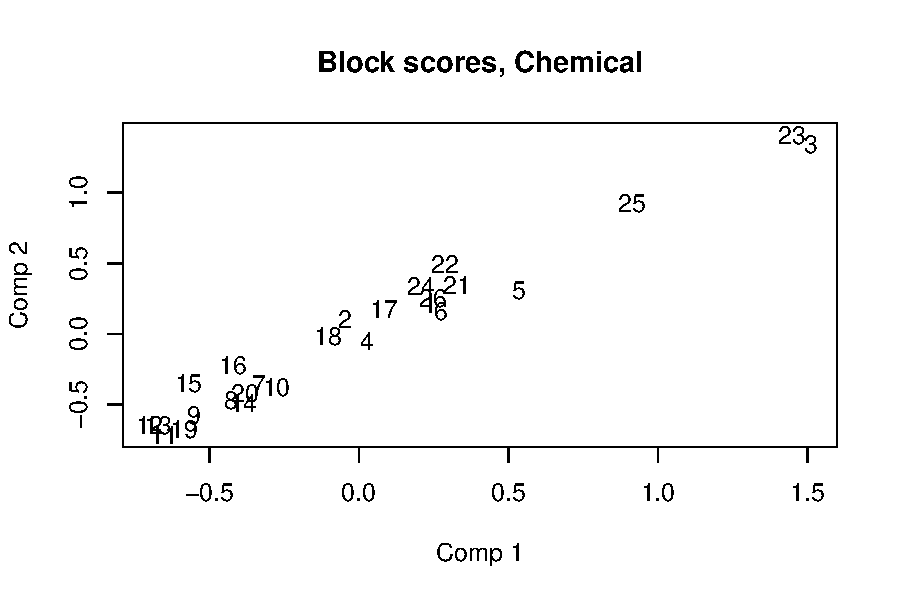
\includegraphics{C:/git/GitHub/multiblock/vignettes/vignette_E_supervised_files/figure-latex/unnamed-chunk-4-1.pdf}

\begin{Shaded}
\begin{Highlighting}[]

\NormalTok{Pb2 }\OtherTok{\textless{}{-}} \FunctionTok{loadings}\NormalTok{(mb, }\AttributeTok{block=}\DecValTok{2}\NormalTok{)}
\FunctionTok{loadingplot}\NormalTok{(mb, }\AttributeTok{block =} \DecValTok{1}\NormalTok{, }\AttributeTok{labels =} \StringTok{"names"}\NormalTok{)}
\end{Highlighting}
\end{Shaded}

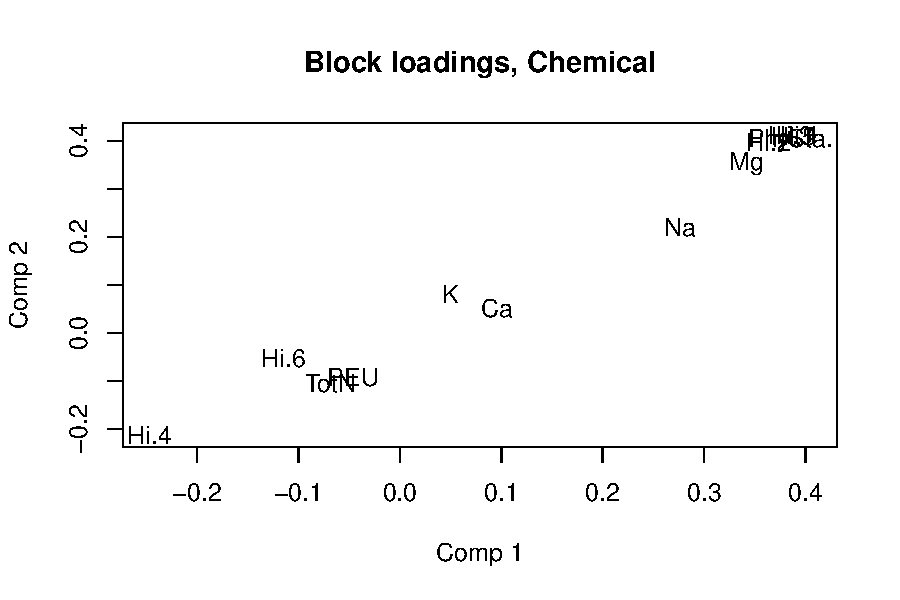
\includegraphics{C:/git/GitHub/multiblock/vignettes/vignette_E_supervised_files/figure-latex/unnamed-chunk-4-2.pdf}

\hypertarget{sparse-multiblock-partial-least-squares---smb-pls}{%
\section{Sparse Multiblock Partial Least Squares -
sMB-PLS}\label{sparse-multiblock-partial-least-squares---smb-pls}}

Sparse MB-PLS is presented briefly using the \emph{potato} data.

\hypertarget{modelling-1}{%
\subsection{Modelling}\label{modelling-1}}

A multi-response two-block sMB-PLS model with up to 10 components in
total is cross-validated with 10 random segments. Here, the
Soft-Threshold version is used (Truncation version also available) with
parameter \emph{shrink = 0.6} means the loading weights have 60\% of the
largest values subtracted before setting negative values to 0.

\begin{Shaded}
\begin{Highlighting}[]
\FunctionTok{data}\NormalTok{(potato)}
\NormalTok{smb }\OtherTok{\textless{}{-}} \FunctionTok{smbpls}\NormalTok{(potato[}\FunctionTok{c}\NormalTok{(}\StringTok{\textquotesingle{}Chemical\textquotesingle{}}\NormalTok{,}\StringTok{\textquotesingle{}Compression\textquotesingle{}}\NormalTok{)], potato[[}\StringTok{\textquotesingle{}Sensory\textquotesingle{}}\NormalTok{]], }\AttributeTok{ncomp =} \DecValTok{10}\NormalTok{,}
            \AttributeTok{max\_comps=}\DecValTok{10}\NormalTok{, }\AttributeTok{shrink =} \FloatTok{0.6}\NormalTok{, }\AttributeTok{validation=}\StringTok{"CV"}\NormalTok{, }\AttributeTok{segments=}\DecValTok{10}\NormalTok{)}
\FunctionTok{print}\NormalTok{(smb)}
\CommentTok{\#\textgreater{} Sparse Multiblock PLS (Soft{-}Threshold) }
\CommentTok{\#\textgreater{} }
\CommentTok{\#\textgreater{} Call:}
\CommentTok{\#\textgreater{} smbpls(X = potato[c("Chemical", "Compression")], Y = potato[["Sensory"]],     ncomp = 10, shrink = 0.6, max\_comps = 10, validation = "CV",     segments = 10)}
\end{Highlighting}
\end{Shaded}

\hypertarget{plotting}{%
\subsection{Plotting}\label{plotting}}

We demonstrate the effect of shrinkage on scores and sparseness in
loading weights by plotting results for three values of the shrinkage
parameter. In the loading weight plots we can follow the shrinkage
toward the origin of each variable, while the score plots show the
effect on the sample scores.

\begin{Shaded}
\begin{Highlighting}[]
\NormalTok{old.par }\OtherTok{\textless{}{-}} \FunctionTok{par}\NormalTok{(}\AttributeTok{mfrow =} \FunctionTok{c}\NormalTok{(}\DecValTok{3}\NormalTok{,}\DecValTok{2}\NormalTok{), }\AttributeTok{mar =} \FunctionTok{c}\NormalTok{(}\FloatTok{3.5}\NormalTok{,}\FloatTok{3.5}\NormalTok{,}\FloatTok{1.5}\NormalTok{,}\DecValTok{1}\NormalTok{), }\AttributeTok{mgp =} \FunctionTok{c}\NormalTok{(}\DecValTok{2}\NormalTok{,}\DecValTok{1}\NormalTok{,}\DecValTok{0}\NormalTok{))}
\ControlFlowTok{for}\NormalTok{(shrink }\ControlFlowTok{in} \FunctionTok{c}\NormalTok{(}\FloatTok{0.2}\NormalTok{, }\FloatTok{0.5}\NormalTok{, }\FloatTok{0.8}\NormalTok{))\{}
\NormalTok{  smb }\OtherTok{\textless{}{-}} \FunctionTok{smbpls}\NormalTok{(potato[}\FunctionTok{c}\NormalTok{(}\StringTok{\textquotesingle{}Chemical\textquotesingle{}}\NormalTok{,}\StringTok{\textquotesingle{}Compression\textquotesingle{}}\NormalTok{)], potato[[}\StringTok{\textquotesingle{}Sensory\textquotesingle{}}\NormalTok{]], }\AttributeTok{ncomp =} \DecValTok{10}\NormalTok{,}
            \AttributeTok{max\_comps=}\DecValTok{10}\NormalTok{, }\AttributeTok{shrink =}\NormalTok{ shrink)}
  \FunctionTok{scoreplot}\NormalTok{(smb, }\AttributeTok{labels =} \StringTok{"names"}\NormalTok{, }\AttributeTok{main =} \FunctionTok{paste0}\NormalTok{(}\StringTok{"Superscores, shrink="}\NormalTok{, shrink))}
  \FunctionTok{loadingweightplot}\NormalTok{(smb, }\AttributeTok{labels =} \StringTok{"names"}\NormalTok{, }\AttributeTok{main =} \FunctionTok{paste0}\NormalTok{(}\StringTok{"Super{-}loading weights, shrink="}\NormalTok{, shrink))}
\NormalTok{\}}
\end{Highlighting}
\end{Shaded}

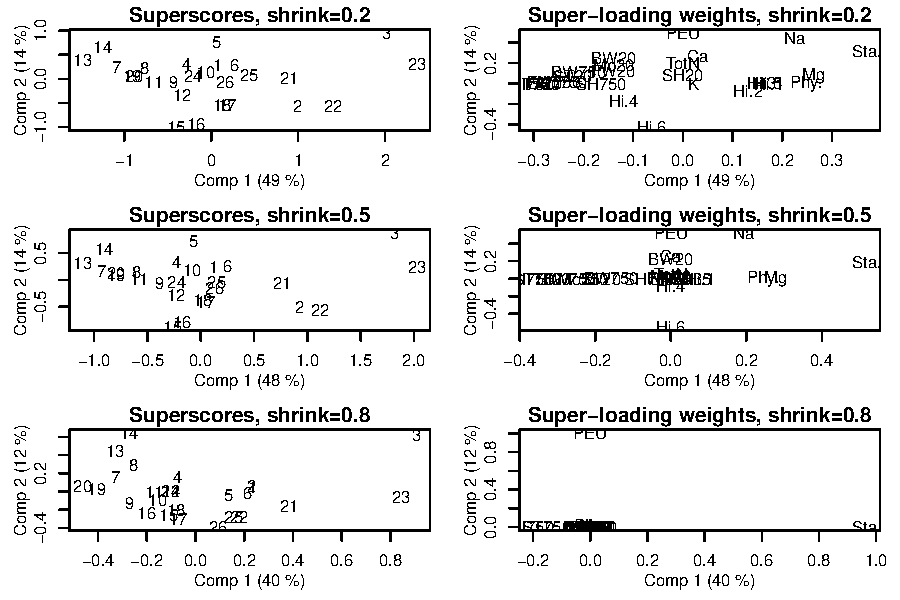
\includegraphics{C:/git/GitHub/multiblock/vignettes/vignette_E_supervised_files/figure-latex/unnamed-chunk-6-1.pdf}

\begin{Shaded}
\begin{Highlighting}[]
\FunctionTok{par}\NormalTok{(old.par)}
\end{Highlighting}
\end{Shaded}

\hypertarget{sequential-and-orthogonalised-pls---so-pls}{%
\section{Sequential and orthogonalised PLS -
SO-PLS}\label{sequential-and-orthogonalised-pls---so-pls}}

The following example uses the \emph{potato} data to showcase some of
the functions available for SO-PLS analyses.

\hypertarget{modelling-2}{%
\subsection{Modelling}\label{modelling-2}}

A multi-response two-block SO-PLS model with up to 10 components in
total is cross-validated with 10 random segments.

\begin{Shaded}
\begin{Highlighting}[]
\CommentTok{\# Load potato data and fit SO{-}PLS model}
\NormalTok{so.pot }\OtherTok{\textless{}{-}} \FunctionTok{sopls}\NormalTok{(Sensory }\SpecialCharTok{\textasciitilde{}}\NormalTok{ Chemical }\SpecialCharTok{+}\NormalTok{ Compression, }\AttributeTok{data=}\NormalTok{potato, }
            \AttributeTok{ncomp=}\FunctionTok{c}\NormalTok{(}\DecValTok{10}\NormalTok{,}\DecValTok{10}\NormalTok{), }\AttributeTok{max\_comps=}\DecValTok{10}\NormalTok{, }\AttributeTok{validation=}\StringTok{"CV"}\NormalTok{, }\AttributeTok{segments=}\DecValTok{10}\NormalTok{)}
\FunctionTok{print}\NormalTok{(so.pot)}
\CommentTok{\#\textgreater{} Sequential and Orthogonalized Partial Least Squares, fitted with the PKPLS algorithm.}
\CommentTok{\#\textgreater{} Cross{-}validated using 10 random segments.}
\CommentTok{\#\textgreater{} Call:}
\CommentTok{\#\textgreater{} sopls(formula = Sensory \textasciitilde{} Chemical + Compression, ncomp = c(10,     10), max\_comps = 10, data = potato, validation = "CV", segments = 10)}
\FunctionTok{summary}\NormalTok{(so.pot)}
\CommentTok{\#\textgreater{} Data:    X dimension: 26 0 }
\CommentTok{\#\textgreater{}  Y dimension: 26 9}
\CommentTok{\#\textgreater{} Fit method: PKPLS}
\CommentTok{\#\textgreater{} Number of components considered: 10}
\CommentTok{\#\textgreater{} }
\CommentTok{\#\textgreater{} VALIDATION: RMSEP}
\CommentTok{\#\textgreater{} Cross{-}validated using 10 random segments.}
\CommentTok{\#\textgreater{}    0,0     0,1     0,2     0,3     0,4     0,5     0,6     0,7     0,8     0,9  }
\CommentTok{\#\textgreater{} 1.1472  0.9974  1.1034  0.9942  1.0159  1.1523  1.0857  1.1834  1.2494  1.3022  }
\CommentTok{\#\textgreater{}   0,10     1,0     1,1     1,2     1,3     1,4     1,5     1,6     1,7     1,8  }
\CommentTok{\#\textgreater{} 1.2690  0.9058  0.8860  0.9779  0.9029  0.8942  0.9320  0.9441  1.0542  1.1243  }
\CommentTok{\#\textgreater{}    1,9     2,0     2,1     2,2     2,3     2,4     2,5     2,6     2,7     2,8  }
\CommentTok{\#\textgreater{} 1.1369  0.8077  0.7023  0.7124  0.7737  0.8072  0.8651  0.8511  0.9742  1.0048  }
\CommentTok{\#\textgreater{}    3,0     3,1     3,2     3,3     3,4     3,5     3,6     3,7     4,0     4,1  }
\CommentTok{\#\textgreater{} 0.7439  0.7275  0.7111  0.7716  0.8322  0.8846  0.8893  0.9793  0.7494  0.7165  }
\CommentTok{\#\textgreater{}    4,2     4,3     4,4     4,5     4,6     5,0     5,1     5,2     5,3     5,4  }
\CommentTok{\#\textgreater{} 0.7272  0.7748  0.8135  0.9157  0.9001  0.7752  0.7491  0.7593  0.8494  0.9693  }
\CommentTok{\#\textgreater{}    5,5     6,0     6,1     6,2     6,3     6,4     7,0     7,1     7,2     7,3  }
\CommentTok{\#\textgreater{} 1.0306  0.8504  0.8438  0.8198  0.9304  1.0222  0.8997  0.8910  0.8418  0.9632  }
\CommentTok{\#\textgreater{}    8,0     8,1     8,2     9,0     9,1    10,0  }
\CommentTok{\#\textgreater{} 1.0062  1.0033  0.9511  1.0682  1.0557  1.6371  }
\CommentTok{\#\textgreater{} }
\CommentTok{\#\textgreater{} TRAINING: \% variance explained}
\CommentTok{\#\textgreater{}         0,0    0,1    0,2    0,3    0,4    0,5    0,6    0,7    0,8    0,9}
\CommentTok{\#\textgreater{} X         0  45.87  55.51  62.90  66.46  67.73  74.95  78.26  79.85  82.39}
\CommentTok{\#\textgreater{} ref       0  42.19  54.73  65.01  66.85  73.96  74.10  74.44  77.45  77.57}
\CommentTok{\#\textgreater{} hard      0  39.11  41.97  42.23  43.80  50.95  54.87  56.78  59.50  74.53}
\CommentTok{\#\textgreater{} firm      0  42.55  57.44  59.44  61.06  66.78  68.62  69.02  71.34  76.53}
\CommentTok{\#\textgreater{} elas      0  38.64  65.31  73.51  75.63  77.23  79.25  81.19  83.71  86.57}
\CommentTok{\#\textgreater{} adhes     0  16.13  18.11  26.71  26.74  29.70  42.07  44.57  46.47  46.54}
\CommentTok{\#\textgreater{} grainy    0  23.21  43.78  62.23  64.02  67.18  67.72  69.83  74.79  74.79}
\CommentTok{\#\textgreater{} mealy     0  35.35  41.99  57.36  58.84  67.17  70.33  73.21  77.77  78.88}
\CommentTok{\#\textgreater{} moist     0  24.48  27.71  43.10  44.27  48.41  53.39  62.37  67.60  74.79}
\CommentTok{\#\textgreater{} chewi     0  21.98  22.78  48.17  55.50  59.96  68.39  72.54  76.39  77.42}
\CommentTok{\#\textgreater{}          0,10    1,0    1,1    1,2    1,3    1,4    1,5    1,6    1,7    1,8}
\CommentTok{\#\textgreater{} X       83.18  34.20  64.12  71.71  76.24  78.20  79.49  83.37  84.42  85.59}
\CommentTok{\#\textgreater{} ref     77.57  55.79  64.00  64.25  73.75  77.39  79.53  80.42  80.50  80.96}
\CommentTok{\#\textgreater{} hard    75.43  24.10  41.42  44.05  44.07  44.09  47.61  53.70  53.86  62.46}
\CommentTok{\#\textgreater{} firm    79.31  42.73  54.16  58.42  62.05  63.55  64.91  70.85  70.91  70.93}
\CommentTok{\#\textgreater{} elas    88.14  53.24  59.32  63.95  71.43  74.51  75.33  77.16  78.86  78.88}
\CommentTok{\#\textgreater{} adhes   54.68  17.49  22.70  33.54  33.75  34.70  34.90  39.43  48.51  48.92}
\CommentTok{\#\textgreater{} grainy  74.82  57.69  58.26  58.39  71.89  75.95  76.07  76.72  77.73  79.00}
\CommentTok{\#\textgreater{} mealy   79.25  61.37  65.64  66.70  74.33  75.36  77.44  78.35  79.55  80.15}
\CommentTok{\#\textgreater{} moist   77.22  57.32  58.51  62.12  66.20  66.35  67.13  67.14  69.51  71.02}
\CommentTok{\#\textgreater{} chewi   81.68  53.27  54.25  64.22  66.35  69.59  69.96  72.80  77.64  77.64}
\CommentTok{\#\textgreater{}           1,9    2,0    2,1    2,2    2,3    2,4    2,5    2,6    2,7    2,8}
\CommentTok{\#\textgreater{} X       86.07  42.76  72.61  79.40  81.41  82.69  84.98  88.16  88.87  89.84}
\CommentTok{\#\textgreater{} ref     81.20  76.03  85.17  87.21  89.03  90.67  90.68  91.36  91.36  91.39}
\CommentTok{\#\textgreater{} hard    69.98  25.29  44.10  46.63  46.63  46.88  52.03  61.89  64.48  73.84}
\CommentTok{\#\textgreater{} firm    80.21  55.93  69.19  76.45  76.45  76.80  77.79  82.58  82.64  86.03}
\CommentTok{\#\textgreater{} elas    87.63  63.10  70.21  78.03  78.08  78.17  80.37  82.19  84.54  85.69}
\CommentTok{\#\textgreater{} adhes   49.97  34.43  39.48  46.70  46.78  48.48  54.50  56.16  67.45  72.74}
\CommentTok{\#\textgreater{} grainy  79.50  83.95  84.78  87.19  88.01  88.56  89.28  89.29  89.30  89.49}
\CommentTok{\#\textgreater{} mealy   80.19  81.14  85.67  85.68  87.94  88.28  88.57  89.15  89.69  90.49}
\CommentTok{\#\textgreater{} moist   72.44  67.94  69.06  70.49  72.51  72.53  72.61  72.80  73.61  78.69}
\CommentTok{\#\textgreater{} chewi   78.05  70.55  71.41  77.11  77.11  78.09  78.17  79.79  83.27  86.51}
\CommentTok{\#\textgreater{}           3,0    3,1    3,2    3,3    3,4    3,5    3,6    3,7    4,0    4,1}
\CommentTok{\#\textgreater{} X       63.76  78.59  84.55  86.77  87.73  90.09  91.81  92.46  70.09  80.35}
\CommentTok{\#\textgreater{} ref     84.50  86.31  87.91  89.34  91.72  91.74  93.12  93.13  84.91  87.28}
\CommentTok{\#\textgreater{} hard    29.51  45.43  50.00  50.23  51.56  54.69  61.12  63.12  30.80  49.39}
\CommentTok{\#\textgreater{} firm    62.42  68.64  76.93  76.96  77.84  78.25  82.67  82.72  62.64  73.46}
\CommentTok{\#\textgreater{} elas    69.44  70.75  78.04  78.06  78.07  80.60  82.75  85.36  69.94  73.16}
\CommentTok{\#\textgreater{} adhes   34.51  46.88  50.83  51.04  51.60  57.45  58.26  69.10  64.76  65.66}
\CommentTok{\#\textgreater{} grainy  87.18  87.45  88.87  89.86  90.34  91.06  91.37  91.45  87.20  87.21}
\CommentTok{\#\textgreater{} mealy   84.89  86.14  86.18  88.32  89.25  89.48  91.02  91.95  88.83  88.96}
\CommentTok{\#\textgreater{} moist   70.03  70.05  72.13  74.57  74.71  74.88  74.97  76.40  75.09  76.33}
\CommentTok{\#\textgreater{} chewi   70.56  72.61  77.34  77.39  78.58  78.58  79.89  83.77  82.06  82.29}
\CommentTok{\#\textgreater{}           4,2    4,3    4,4    4,5    4,6    5,0    5,1    5,2    5,3    5,4}
\CommentTok{\#\textgreater{} X       87.12  88.89  89.78  92.03  93.37  75.21  84.27  91.16  92.52  93.47}
\CommentTok{\#\textgreater{} ref     88.13  89.65  92.48  92.54  93.63  85.03  88.23  89.16  90.27  92.85}
\CommentTok{\#\textgreater{} hard    49.95  50.65  50.76  54.96  60.99  41.38  53.88  54.08  54.33  54.70}
\CommentTok{\#\textgreater{} firm    77.00  77.10  77.44  78.23  83.34  68.24  75.97  78.78  78.78  79.40}
\CommentTok{\#\textgreater{} elas    78.98  79.09  79.43  82.78  83.85  72.35  74.56  79.87  80.48  80.91}
\CommentTok{\#\textgreater{} adhes   67.28  68.26  69.21  70.41  70.90  64.77  65.81  67.35  67.83  69.01}
\CommentTok{\#\textgreater{} grainy  89.07  90.46  91.63  92.15  92.30  87.53  87.56  89.67  90.98  91.93}
\CommentTok{\#\textgreater{} mealy   88.99  93.13  94.52  94.64  95.00  89.21  89.65  89.73  93.45  94.51}
\CommentTok{\#\textgreater{} moist   76.60  82.33  82.90  82.90  83.28  79.72  79.91  79.98  83.86  84.08}
\CommentTok{\#\textgreater{} chewi   84.08  84.45  86.24  86.38  86.39  82.11  82.31  83.97  84.76  86.45}
\CommentTok{\#\textgreater{}           5,5    6,0    6,1    6,2    6,3    6,4    7,0    7,1    7,2    7,3}
\CommentTok{\#\textgreater{} X       95.40  77.28  86.22  93.18  94.55  95.63  79.57  88.43  95.46  96.65}
\CommentTok{\#\textgreater{} ref     92.91  86.80  90.43  91.47  92.26  94.07  88.07  91.60  92.62  92.70}
\CommentTok{\#\textgreater{} hard    60.53  45.27  56.94  57.05  57.64  59.71  45.28  56.91  56.99  57.22}
\CommentTok{\#\textgreater{} firm    80.75  68.98  76.56  79.17  79.42  80.55  69.02  76.72  79.16  79.35}
\CommentTok{\#\textgreater{} elas    83.34  72.55  74.96  80.08  80.15  80.26  73.76  76.39  81.36  81.61}
\CommentTok{\#\textgreater{} adhes   70.53  64.77  65.79  67.29  69.17  69.37  65.04  65.96  67.53  68.89}
\CommentTok{\#\textgreater{} grainy  92.38  91.29  91.41  93.80  94.06  94.27  91.78  91.89  94.29  94.34}
\CommentTok{\#\textgreater{} mealy   94.83  90.67  91.24  91.36  94.83  95.44  92.38  92.87  92.98  94.77}
\CommentTok{\#\textgreater{} moist   84.08  82.80  82.90  82.93  85.65  85.67  85.12  85.26  85.29  86.55}
\CommentTok{\#\textgreater{} chewi   86.50  84.60  84.72  86.16  86.49  87.50  86.05  86.22  87.61  87.62}
\CommentTok{\#\textgreater{}           8,0    8,1    8,2    9,0    9,1   10,0}
\CommentTok{\#\textgreater{} X       82.82  88.16  95.96  85.49  90.21  87.08}
\CommentTok{\#\textgreater{} ref     90.82  94.67  94.93  91.52  94.42  91.79}
\CommentTok{\#\textgreater{} hard    52.73  59.90  60.33  52.75  63.37  52.92}
\CommentTok{\#\textgreater{} firm    71.26  80.42  80.49  71.81  80.88  71.82}
\CommentTok{\#\textgreater{} elas    73.78  80.71  81.41  75.22  80.15  76.14}
\CommentTok{\#\textgreater{} adhes   68.88  68.89  69.28  71.74  72.73  74.17}
\CommentTok{\#\textgreater{} grainy  91.80  93.21  94.39  91.99  92.91  92.43}
\CommentTok{\#\textgreater{} mealy   93.59  94.05  94.31  93.75  93.98  93.83}
\CommentTok{\#\textgreater{} moist   86.40  86.60  87.34  87.11  88.40  87.14}
\CommentTok{\#\textgreater{} chewi   87.11  88.40  88.43  87.27  89.53  87.28}
\end{Highlighting}
\end{Shaded}

\hypertarget{muxe5ge-plot}{%
\subsection{Måge plot}\label{muxe5ge-plot}}

Full Måge plot for all combinations of components for all blocks. This
can be used for a global search for the best fitting cross-validated
model.

Each point in the figure below is accompanied by a sequence of four
numbers referring to the number of components used for each of the four
blocks. Horizontal location is given by the total number of components
used across all blocks, while vertical location indicates validated
explained variance in percentage.

\begin{Shaded}
\begin{Highlighting}[]
\CommentTok{\# Load Wine data and model with SO{-}PLS}
\FunctionTok{data}\NormalTok{(wine)}
\NormalTok{ncomp }\OtherTok{\textless{}{-}} \FunctionTok{unlist}\NormalTok{(}\FunctionTok{lapply}\NormalTok{(wine, ncol))[}\SpecialCharTok{{-}}\DecValTok{5}\NormalTok{]}
\NormalTok{so.wine }\OtherTok{\textless{}{-}} \FunctionTok{sopls}\NormalTok{(}\StringTok{\textasciigrave{}}\AttributeTok{Global quality}\StringTok{\textasciigrave{}} \SpecialCharTok{\textasciitilde{}}\NormalTok{ ., }\AttributeTok{data=}\NormalTok{wine, }\AttributeTok{ncomp=}\NormalTok{ncomp, }
             \AttributeTok{max\_comps=}\DecValTok{6}\NormalTok{, }\AttributeTok{validation=}\StringTok{"CV"}\NormalTok{, }\AttributeTok{segments=}\DecValTok{10}\NormalTok{)}
\FunctionTok{maage}\NormalTok{(so.wine)}
\end{Highlighting}
\end{Shaded}

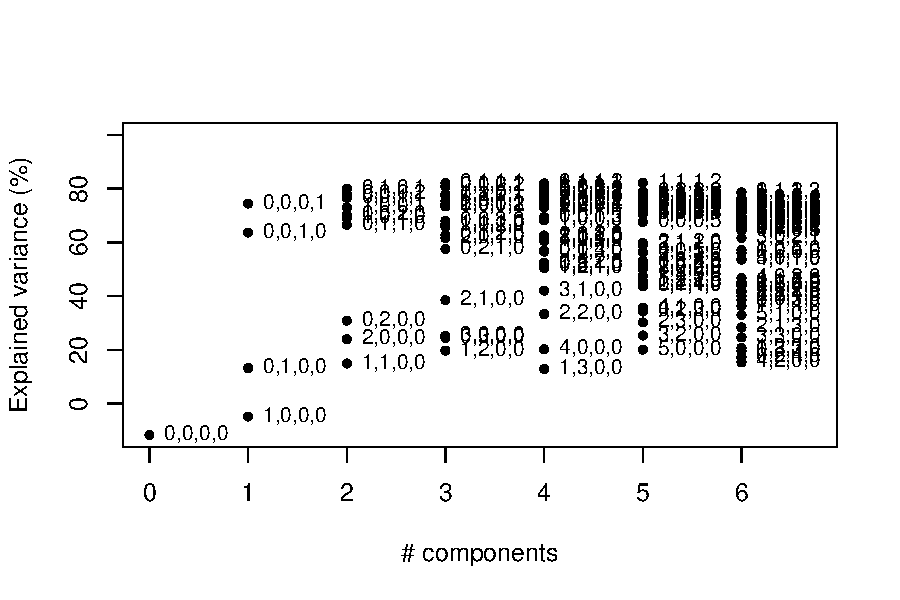
\includegraphics{C:/git/GitHub/multiblock/vignettes/vignette_E_supervised_files/figure-latex/unnamed-chunk-8-1.pdf}

A sequential Måge plot can be used for a sequential search for the
optimal model.

\begin{Shaded}
\begin{Highlighting}[]
\CommentTok{\# Sequential search for optimal number of components per block}
\NormalTok{old.par }\OtherTok{\textless{}{-}} \FunctionTok{par}\NormalTok{(}\AttributeTok{mfrow=}\FunctionTok{c}\NormalTok{(}\DecValTok{2}\NormalTok{,}\DecValTok{2}\NormalTok{), }\AttributeTok{mar=}\FunctionTok{c}\NormalTok{(}\DecValTok{3}\NormalTok{,}\DecValTok{3}\NormalTok{,}\FloatTok{0.5}\NormalTok{,}\DecValTok{1}\NormalTok{), }\AttributeTok{mgp=}\FunctionTok{c}\NormalTok{(}\DecValTok{2}\NormalTok{,}\FloatTok{0.7}\NormalTok{,}\DecValTok{0}\NormalTok{))}
\FunctionTok{maageSeq}\NormalTok{(so.wine)}
\FunctionTok{maageSeq}\NormalTok{(so.wine, }\DecValTok{2}\NormalTok{)}
\FunctionTok{maageSeq}\NormalTok{(so.wine, }\FunctionTok{c}\NormalTok{(}\DecValTok{2}\NormalTok{,}\DecValTok{1}\NormalTok{))}
\FunctionTok{maageSeq}\NormalTok{(so.wine, }\FunctionTok{c}\NormalTok{(}\DecValTok{2}\NormalTok{,}\DecValTok{1}\NormalTok{,}\DecValTok{1}\NormalTok{))}
\end{Highlighting}
\end{Shaded}

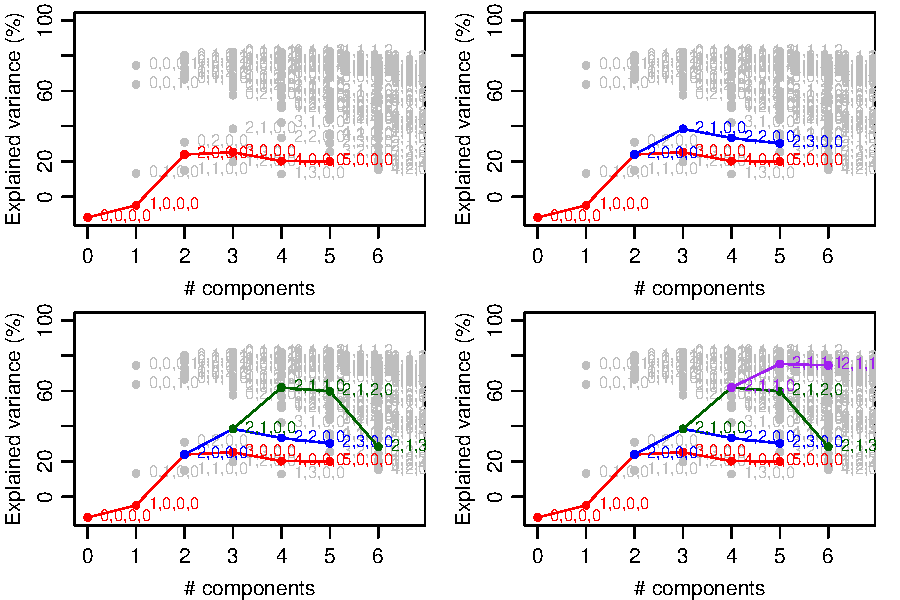
\includegraphics{C:/git/GitHub/multiblock/vignettes/vignette_E_supervised_files/figure-latex/unnamed-chunk-9-1.pdf}

\begin{Shaded}
\begin{Highlighting}[]
\FunctionTok{par}\NormalTok{(old.par)}
\end{Highlighting}
\end{Shaded}

\hypertarget{loadings}{%
\subsection{Loadings}\label{loadings}}

One set of loadings is printed and two sets are plotted to show how to
select specific components from specific blocks. When extracting or
plotting loadings for the second or later blocks, one must specify how
many components have been used in the previous block as this will affect
the choice of loadings.

\begin{Shaded}
\begin{Highlighting}[]
\CommentTok{\# Display loadings for first block}
\FunctionTok{loadings}\NormalTok{(so.pot, }\AttributeTok{block =} \DecValTok{1}\NormalTok{)}
\CommentTok{\#\textgreater{} }
\CommentTok{\#\textgreater{} Loadings:}
\CommentTok{\#\textgreater{}              1,0    2,0    3,0    4,0    5,0    6,0    7,0    8,0    9,0   }
\CommentTok{\#\textgreater{} ChemicalPEU   0.645 {-}3.672  1.197  2.277 {-}0.589 {-}1.684  1.028  0.431  0.118}
\CommentTok{\#\textgreater{} ChemicalSta. {-}4.542 {-}0.975 {-}0.984 {-}0.678 {-}0.559 {-}0.926 {-}0.418 {-}0.583  0.508}
\CommentTok{\#\textgreater{} ChemicalTotN  0.478 {-}1.848  3.046 {-}1.613  1.604 {-}1.088  1.441  0.355 {-}1.874}
\CommentTok{\#\textgreater{} ChemicalPhy. {-}3.970        {-}1.445  0.948  1.148 {-}0.286  1.519 {-}0.669  0.233}
\CommentTok{\#\textgreater{} ChemicalCa   {-}1.365 {-}0.982  1.804 {-}1.190 {-}3.763  1.249  0.107  0.281 {-}0.401}
\CommentTok{\#\textgreater{} ChemicalMg   {-}4.009 {-}0.280        {-}2.344  0.996 {-}0.320  1.152  0.172  0.801}
\CommentTok{\#\textgreater{} ChemicalNa   {-}3.066 {-}2.488  0.669  1.616 {-}1.119  1.520 {-}0.570 {-}0.430 {-}0.452}
\CommentTok{\#\textgreater{} ChemicalK    {-}0.186 {-}0.255 {-}4.161  0.149  0.700  1.225 {-}1.469  1.284 {-}1.263}
\CommentTok{\#\textgreater{} ChemicalHi.1 {-}4.493  2.113         0.344 {-}0.226        {-}0.126  0.108 {-}0.154}
\CommentTok{\#\textgreater{} ChemicalHi.2 {-}4.099  2.656 {-}0.739  0.488 {-}0.311 {-}0.225  0.135  0.120 {-}0.254}
\CommentTok{\#\textgreater{} ChemicalHi.3 {-}4.382  2.270 {-}0.259  0.398 {-}0.272 {-}0.271  0.105  0.337 {-}0.369}
\CommentTok{\#\textgreater{} ChemicalHi.4  3.000  0.732 {-}2.855        {-}1.994 {-}0.483  1.552 {-}0.173 {-}0.200}
\CommentTok{\#\textgreater{} ChemicalHi.5 {-}4.419  2.023 {-}0.177  0.372 {-}0.362 {-}0.359  0.192  0.494 {-}0.668}
\CommentTok{\#\textgreater{} ChemicalHi.6  1.580  2.266 {-}3.570  0.571 {-}1.131 {-}0.664  1.351 {-}0.390 {-}0.371}
\CommentTok{\#\textgreater{}              10,0  }
\CommentTok{\#\textgreater{} ChemicalPEU  {-}0.132}
\CommentTok{\#\textgreater{} ChemicalSta.  0.220}
\CommentTok{\#\textgreater{} ChemicalTotN       }
\CommentTok{\#\textgreater{} ChemicalPhy. {-}1.415}
\CommentTok{\#\textgreater{} ChemicalCa   {-}1.229}
\CommentTok{\#\textgreater{} ChemicalMg    0.481}
\CommentTok{\#\textgreater{} ChemicalNa    1.440}
\CommentTok{\#\textgreater{} ChemicalK    {-}0.411}
\CommentTok{\#\textgreater{} ChemicalHi.1  0.162}
\CommentTok{\#\textgreater{} ChemicalHi.2  0.146}
\CommentTok{\#\textgreater{} ChemicalHi.3       }
\CommentTok{\#\textgreater{} ChemicalHi.4  0.528}
\CommentTok{\#\textgreater{} ChemicalHi.5       }
\CommentTok{\#\textgreater{} ChemicalHi.6  0.279}
\CommentTok{\#\textgreater{} }
\CommentTok{\#\textgreater{}                    1,0    2,0    3,0    4,0    5,0    6,0    7,0    8,0    9,0}
\CommentTok{\#\textgreater{} SS loadings    151.624 51.586 56.326 19.671 27.054 11.370 13.749  3.605  7.288}
\CommentTok{\#\textgreater{} Proportion Var  10.830  3.685  4.023  1.405  1.932  0.812  0.982  0.257  0.521}
\CommentTok{\#\textgreater{} Cumulative Var  10.830 14.515 18.538 19.943 21.876 22.688 23.670 23.927 24.448}
\CommentTok{\#\textgreater{}                  10,0}
\CommentTok{\#\textgreater{} SS loadings     6.470}
\CommentTok{\#\textgreater{} Proportion Var  0.462}
\CommentTok{\#\textgreater{} Cumulative Var 24.910}
\end{Highlighting}
\end{Shaded}

\begin{Shaded}
\begin{Highlighting}[]
\CommentTok{\# Plot loadings from block 1 and 2}
\NormalTok{old.par }\OtherTok{\textless{}{-}} \FunctionTok{par}\NormalTok{(}\AttributeTok{mfrow=}\FunctionTok{c}\NormalTok{(}\DecValTok{1}\NormalTok{,}\DecValTok{2}\NormalTok{))}
\FunctionTok{loadingplot}\NormalTok{(so.pot, }\AttributeTok{comps =} \FunctionTok{c}\NormalTok{(}\DecValTok{2}\NormalTok{,}\DecValTok{3}\NormalTok{), }\AttributeTok{block =} \DecValTok{1}\NormalTok{, }\AttributeTok{main =} \StringTok{"Block 1"}\NormalTok{, }\AttributeTok{labels =} \StringTok{"names"}\NormalTok{, }\AttributeTok{cex =} \FloatTok{0.8}\NormalTok{)}
\FunctionTok{loadingplot}\NormalTok{(so.pot, }\AttributeTok{ncomp =} \DecValTok{4}\NormalTok{, }\AttributeTok{block =} \DecValTok{2}\NormalTok{, }\AttributeTok{main =} \StringTok{"Block 2"}\NormalTok{, }\AttributeTok{labels =} \StringTok{"names"}\NormalTok{, }\AttributeTok{cex =} \FloatTok{0.8}\NormalTok{)}
\end{Highlighting}
\end{Shaded}

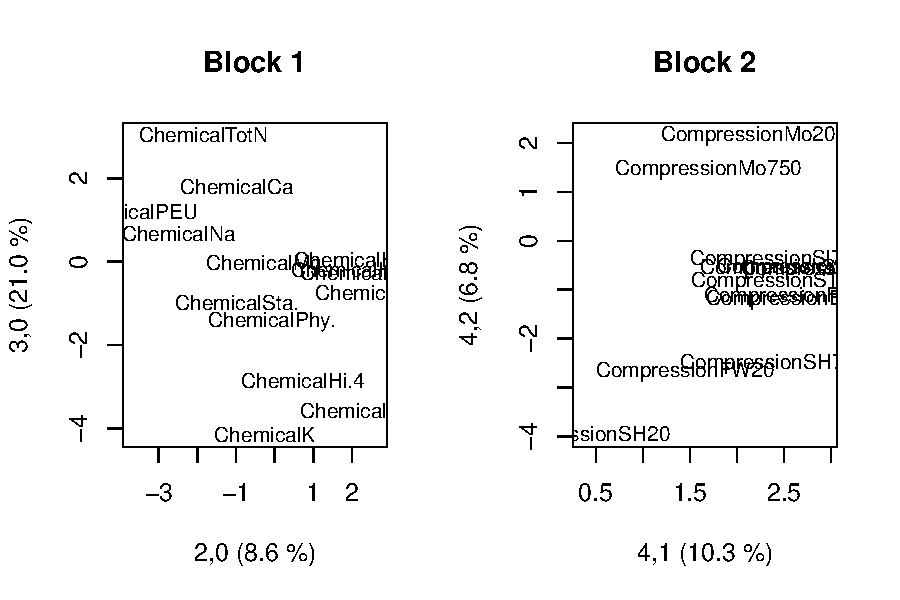
\includegraphics{C:/git/GitHub/multiblock/vignettes/vignette_E_supervised_files/figure-latex/unnamed-chunk-11-1.pdf}

\begin{Shaded}
\begin{Highlighting}[]
\FunctionTok{par}\NormalTok{(old.par)}
\end{Highlighting}
\end{Shaded}

\hypertarget{scores}{%
\subsection{Scores}\label{scores}}

One set of scores is printed and two sets are plotted to show how to
select specific components from specific blocks. Specification of
component use in preceding blocks follows the same pattern as with
loadings.

\begin{Shaded}
\begin{Highlighting}[]
\CommentTok{\# Display scores for first block}
\FunctionTok{scores}\NormalTok{(so.pot, }\AttributeTok{block =} \DecValTok{1}\NormalTok{)}
\CommentTok{\#\textgreater{}             1,0         2,0          3,0         4,0         5,0          6,0}
\CommentTok{\#\textgreater{} 1  {-}0.078379126 {-}0.15756558 {-}0.030150796 {-}0.08882899 {-}0.01376296 {-}0.056671801}
\CommentTok{\#\textgreater{} 2   0.033599245  0.03345139 {-}0.264837392 {-}0.02082345 {-}0.11717078 {-}0.151392736}
\CommentTok{\#\textgreater{} 3  {-}0.454087240 {-}0.50387774 {-}0.257625630  0.24822188 {-}0.02903093 {-}0.086528935}
\CommentTok{\#\textgreater{} 4  {-}0.010144029  0.04409907  0.254739277  0.34206013  0.02495265  0.074552441}
\CommentTok{\#\textgreater{} 5  {-}0.231320589  0.02813994  0.331647163 {-}0.15209020 {-}0.75827354  0.341572360}
\CommentTok{\#\textgreater{} 6  {-}0.100806072 {-}0.03203490  0.058511494 {-}0.07824489 {-}0.03272086  0.022355259}
\CommentTok{\#\textgreater{} 7   0.103759602  0.05587580  0.171495995  0.13245956 {-}0.01979756 {-}0.159062060}
\CommentTok{\#\textgreater{} 8   0.142341829 {-}0.02952316  0.135315864  0.17766566 {-}0.04381490 {-}0.186272842}
\CommentTok{\#\textgreater{} 9   0.160175421 {-}0.13395363  0.067732083 {-}0.34567441  0.17107748  0.172779015}
\CommentTok{\#\textgreater{} 10  0.078862890 {-}0.20282246  0.065251294 {-}0.21205811  0.20044571  0.328237338}
\CommentTok{\#\textgreater{} 11  0.200245777 {-}0.02882659  0.149667777 {-}0.08872396 {-}0.08768916 {-}0.174332305}
\CommentTok{\#\textgreater{} 12  0.223602068 {-}0.07321286 {-}0.029748834 {-}0.22950703 {-}0.03709102 {-}0.193124707}
\CommentTok{\#\textgreater{} 13  0.217320106 {-}0.26815383  0.096949900 {-}0.10070260  0.05733144 {-}0.253089620}
\CommentTok{\#\textgreater{} 14  0.142847549 {-}0.29951537  0.077252287  0.24996525 {-}0.11362892 {-}0.187257376}
\CommentTok{\#\textgreater{} 15  0.213820293  0.17228886 {-}0.461863019 {-}0.11767172 {-}0.27195381 {-}0.069378444}
\CommentTok{\#\textgreater{} 16  0.164964325  0.26005269 {-}0.323577542  0.10235857 {-}0.18083698  0.028860577}
\CommentTok{\#\textgreater{} 17  0.002967383  0.19480792 {-}0.246885356  0.19701818  0.05083294  0.193040181}
\CommentTok{\#\textgreater{} 18  0.066258347  0.09356886 {-}0.228532411  0.20484080  0.06435515  0.193713440}
\CommentTok{\#\textgreater{} 19  0.194213760 {-}0.01568159  0.132000297  0.14447620  0.07380230  0.134307084}
\CommentTok{\#\textgreater{} 20  0.141301554 {-}0.07654188  0.049224760  0.26084474  0.16978368  0.406994445}
\CommentTok{\#\textgreater{} 21 {-}0.129888279  0.04471652  0.038982799 {-}0.30565064  0.07729299 {-}0.272193959}
\CommentTok{\#\textgreater{} 22 {-}0.105636544  0.24576605 {-}0.030041538 {-}0.14535670  0.24832087  0.010288729}
\CommentTok{\#\textgreater{} 23 {-}0.464479945 {-}0.11433433 {-}0.194275154 {-}0.06714686  0.13063332 {-}0.005785022}
\CommentTok{\#\textgreater{} 24 {-}0.082441922  0.22751259  0.233417343  0.13675311  0.22568931 {-}0.091378804}
\CommentTok{\#\textgreater{} 25 {-}0.325181587  0.44765983  0.208213841  0.07217114  0.05115869 {-}0.267361478}
\CommentTok{\#\textgreater{} 26 {-}0.103914818  0.08810440 {-}0.002864502 {-}0.31635566  0.16009487  0.247129222}
\CommentTok{\#\textgreater{}             7,0          8,0         9,0         10,0}
\CommentTok{\#\textgreater{} 1  {-}0.170176673 {-}0.353657625  0.09144069 {-}0.188197767}
\CommentTok{\#\textgreater{} 2   0.376363608 {-}0.223166913 {-}0.06432803  0.102154561}
\CommentTok{\#\textgreater{} 3   0.053642203  0.053088656  0.11136825  0.089274658}
\CommentTok{\#\textgreater{} 4   0.080021975 {-}0.455836399  0.29151166  0.160435908}
\CommentTok{\#\textgreater{} 5   0.060316124  0.088814534 {-}0.01259842 {-}0.241887363}
\CommentTok{\#\textgreater{} 6  {-}0.143868448  0.209487156  0.44247087  0.460290223}
\CommentTok{\#\textgreater{} 7  {-}0.067499572  0.172789197 {-}0.01007070  0.014280187}
\CommentTok{\#\textgreater{} 8   0.003023123  0.020901351 {-}0.15855793  0.115799243}
\CommentTok{\#\textgreater{} 9   0.099124600  0.077168263 {-}0.22926057  0.020019625}
\CommentTok{\#\textgreater{} 10 {-}0.006546077  0.001048562 {-}0.15821313  0.090958585}
\CommentTok{\#\textgreater{} 11 {-}0.321845257 {-}0.388050068 {-}0.15769574  0.033224651}
\CommentTok{\#\textgreater{} 12 {-}0.114302438 {-}0.157344716  0.01456158 {-}0.118230072}
\CommentTok{\#\textgreater{} 13  0.159102296  0.426179096  0.31221443 {-}0.244022144}
\CommentTok{\#\textgreater{} 14  0.164565349  0.160117465 {-}0.31148972  0.004138940}
\CommentTok{\#\textgreater{} 15  0.160269738 {-}0.034424824  0.04760954  0.177518448}
\CommentTok{\#\textgreater{} 16  0.073035199  0.028396505  0.02512587  0.008674474}
\CommentTok{\#\textgreater{} 17 {-}0.336494502  0.228154141 {-}0.02760929 {-}0.191196309}
\CommentTok{\#\textgreater{} 18 {-}0.353315626  0.070825686  0.13990043 {-}0.255631862}
\CommentTok{\#\textgreater{} 19 {-}0.192020302  0.118534017 {-}0.05488875  0.206887988}
\CommentTok{\#\textgreater{} 20  0.167499146 {-}0.065961803 {-}0.17176149 {-}0.018385084}
\CommentTok{\#\textgreater{} 21 {-}0.291917226 {-}0.005778312  0.06774798 {-}0.093267865}
\CommentTok{\#\textgreater{} 22  0.315505112  0.055322691 {-}0.04212437 {-}0.272120565}
\CommentTok{\#\textgreater{} 23 {-}0.070388026 {-}0.103937894 {-}0.28625584 {-}0.102958571}
\CommentTok{\#\textgreater{} 24  0.271169417 {-}0.112282869  0.28534458 {-}0.337006550}
\CommentTok{\#\textgreater{} 25 {-}0.033293058  0.199555988 {-}0.33284978  0.259557484}
\CommentTok{\#\textgreater{} 26  0.118029313 {-}0.009941885  0.18840789  0.319689179}
\CommentTok{\#\textgreater{} attr(,"explvar")}
\CommentTok{\#\textgreater{}       1,0       2,0       3,0       4,0       5,0       6,0       7,0       8,0 }
\CommentTok{\#\textgreater{} 34.201725  8.556741 20.999993  6.330308  5.124745  2.071311  2.284023  3.250427 }
\CommentTok{\#\textgreater{}       9,0      10,0 }
\CommentTok{\#\textgreater{}  2.674759  1.582372 }
\CommentTok{\#\textgreater{} attr(,"class")}
\CommentTok{\#\textgreater{} [1] "scores.multiblock" "scores"}
\end{Highlighting}
\end{Shaded}

\begin{Shaded}
\begin{Highlighting}[]
\CommentTok{\# Plot scores from block 1 and 2}
\NormalTok{old.par }\OtherTok{\textless{}{-}} \FunctionTok{par}\NormalTok{(}\AttributeTok{mfrow=}\FunctionTok{c}\NormalTok{(}\DecValTok{1}\NormalTok{,}\DecValTok{2}\NormalTok{))}
\FunctionTok{scoreplot}\NormalTok{(so.pot, }\AttributeTok{comps =} \FunctionTok{c}\NormalTok{(}\DecValTok{2}\NormalTok{,}\DecValTok{3}\NormalTok{), }\AttributeTok{block =} \DecValTok{1}\NormalTok{, }\AttributeTok{main =} \StringTok{"Block 1"}\NormalTok{, }\AttributeTok{labels =} \StringTok{"names"}\NormalTok{)}
\FunctionTok{scoreplot}\NormalTok{(so.pot, }\AttributeTok{ncomp =} \DecValTok{4}\NormalTok{, }\AttributeTok{block =} \DecValTok{2}\NormalTok{, }\AttributeTok{main =} \StringTok{"Block 2"}\NormalTok{, }\AttributeTok{labels =} \StringTok{"names"}\NormalTok{)}
\end{Highlighting}
\end{Shaded}

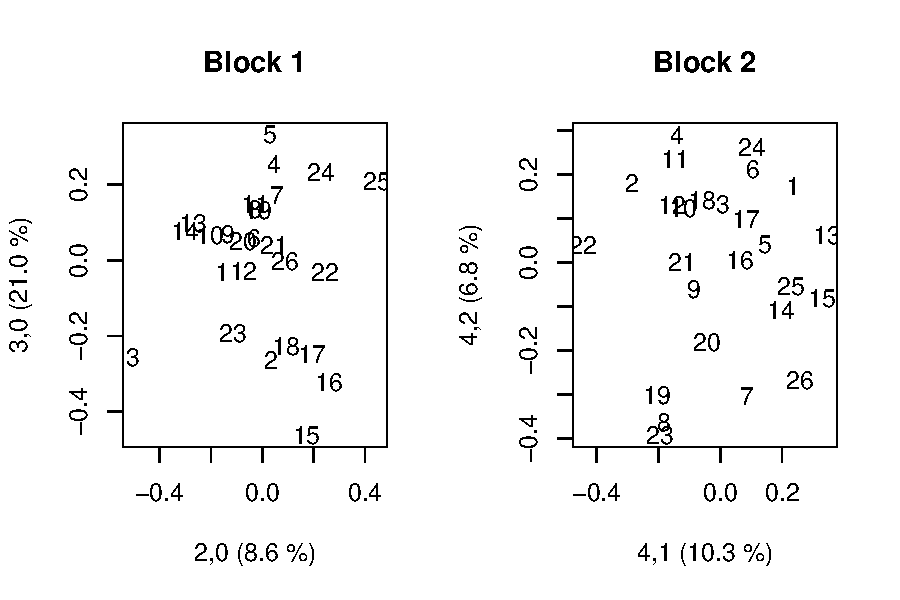
\includegraphics{C:/git/GitHub/multiblock/vignettes/vignette_E_supervised_files/figure-latex/unnamed-chunk-13-1.pdf}

\begin{Shaded}
\begin{Highlighting}[]
\FunctionTok{par}\NormalTok{(old.par)}
\end{Highlighting}
\end{Shaded}

\hypertarget{prediction}{%
\subsection{Prediction}\label{prediction}}

A three block model is fitted using a single response, 5 components and
a subset of the data. The remaining data are used as test set for
prediction.

\begin{Shaded}
\begin{Highlighting}[]
\CommentTok{\# Modify data to contain a single response}
\NormalTok{potato1 }\OtherTok{\textless{}{-}}\NormalTok{ potato; potato1}\SpecialCharTok{$}\NormalTok{Sensory }\OtherTok{\textless{}{-}}\NormalTok{ potato1}\SpecialCharTok{$}\NormalTok{Sensory[,}\DecValTok{1}\NormalTok{]}
\CommentTok{\# Model 20 first objects with SO{-}PLS}
\NormalTok{so.pot20 }\OtherTok{\textless{}{-}} \FunctionTok{sopls}\NormalTok{(Sensory }\SpecialCharTok{\textasciitilde{}}\NormalTok{ ., }\AttributeTok{data =}\NormalTok{ potato1[}\FunctionTok{c}\NormalTok{(}\DecValTok{1}\SpecialCharTok{:}\DecValTok{3}\NormalTok{,}\DecValTok{9}\NormalTok{)], }\AttributeTok{ncomp =} \DecValTok{5}\NormalTok{, }\AttributeTok{subset =} \DecValTok{1}\SpecialCharTok{:}\DecValTok{20}\NormalTok{)}
\CommentTok{\# Predict remaining objects}
\NormalTok{testset }\OtherTok{\textless{}{-}}\NormalTok{ potato1[}\SpecialCharTok{{-}}\NormalTok{(}\DecValTok{1}\SpecialCharTok{:}\DecValTok{20}\NormalTok{),]; }\CommentTok{\# testset$Sensory \textless{}{-} NULL}
\FunctionTok{predict}\NormalTok{(so.pot20, testset, }\AttributeTok{comps=}\FunctionTok{c}\NormalTok{(}\DecValTok{2}\NormalTok{,}\DecValTok{1}\NormalTok{,}\DecValTok{2}\NormalTok{))}
\CommentTok{\#\textgreater{} , , 1,0,0}
\CommentTok{\#\textgreater{} }
\CommentTok{\#\textgreater{}       Sensory}
\CommentTok{\#\textgreater{} [1,] 3.710097}
\CommentTok{\#\textgreater{} [2,] 3.508955}
\CommentTok{\#\textgreater{} [3,] 6.066989}
\CommentTok{\#\textgreater{} [4,] 3.521423}
\CommentTok{\#\textgreater{} [5,] 4.944123}
\CommentTok{\#\textgreater{} [6,] 3.539052}
\CommentTok{\#\textgreater{} }
\CommentTok{\#\textgreater{} , , 2,0,0}
\CommentTok{\#\textgreater{} }
\CommentTok{\#\textgreater{}       Sensory}
\CommentTok{\#\textgreater{} [1,] 3.636431}
\CommentTok{\#\textgreater{} [2,] 3.610855}
\CommentTok{\#\textgreater{} [3,] 6.429357}
\CommentTok{\#\textgreater{} [4,] 3.393957}
\CommentTok{\#\textgreater{} [5,] 4.062585}
\CommentTok{\#\textgreater{} [6,] 3.449857}
\CommentTok{\#\textgreater{} }
\CommentTok{\#\textgreater{} , , 3,0,0}
\CommentTok{\#\textgreater{} }
\CommentTok{\#\textgreater{}       Sensory}
\CommentTok{\#\textgreater{} [1,] 3.688660}
\CommentTok{\#\textgreater{} [2,] 3.685508}
\CommentTok{\#\textgreater{} [3,] 6.480693}
\CommentTok{\#\textgreater{} [4,] 3.211579}
\CommentTok{\#\textgreater{} [5,] 3.956964}
\CommentTok{\#\textgreater{} [6,] 3.464106}
\CommentTok{\#\textgreater{} }
\CommentTok{\#\textgreater{} , , 4,0,0}
\CommentTok{\#\textgreater{} }
\CommentTok{\#\textgreater{}       Sensory}
\CommentTok{\#\textgreater{} [1,] 3.746689}
\CommentTok{\#\textgreater{} [2,] 3.545318}
\CommentTok{\#\textgreater{} [3,] 6.342659}
\CommentTok{\#\textgreater{} [4,] 2.980819}
\CommentTok{\#\textgreater{} [5,] 3.631846}
\CommentTok{\#\textgreater{} [6,] 3.419858}
\CommentTok{\#\textgreater{} }
\CommentTok{\#\textgreater{} , , 5,0,0}
\CommentTok{\#\textgreater{} }
\CommentTok{\#\textgreater{}       Sensory}
\CommentTok{\#\textgreater{} [1,] 3.741608}
\CommentTok{\#\textgreater{} [2,] 3.034433}
\CommentTok{\#\textgreater{} [3,] 6.123613}
\CommentTok{\#\textgreater{} [4,] 2.363783}
\CommentTok{\#\textgreater{} [5,] 2.979181}
\CommentTok{\#\textgreater{} [6,] 3.078927}
\CommentTok{\#\textgreater{} }
\CommentTok{\#\textgreater{} , , 5,1,0}
\CommentTok{\#\textgreater{} }
\CommentTok{\#\textgreater{}       Sensory}
\CommentTok{\#\textgreater{} [1,] 3.636086}
\CommentTok{\#\textgreater{} [2,] 2.582345}
\CommentTok{\#\textgreater{} [3,] 6.196188}
\CommentTok{\#\textgreater{} [4,] 1.914878}
\CommentTok{\#\textgreater{} [5,] 2.804766}
\CommentTok{\#\textgreater{} [6,] 3.092452}
\CommentTok{\#\textgreater{} }
\CommentTok{\#\textgreater{} , , 5,2,0}
\CommentTok{\#\textgreater{} }
\CommentTok{\#\textgreater{}       Sensory}
\CommentTok{\#\textgreater{} [1,] 3.847071}
\CommentTok{\#\textgreater{} [2,] 3.105369}
\CommentTok{\#\textgreater{} [3,] 6.731938}
\CommentTok{\#\textgreater{} [4,] 1.914845}
\CommentTok{\#\textgreater{} [5,] 2.913156}
\CommentTok{\#\textgreater{} [6,] 3.201600}
\CommentTok{\#\textgreater{} }
\CommentTok{\#\textgreater{} , , 5,3,0}
\CommentTok{\#\textgreater{} }
\CommentTok{\#\textgreater{}       Sensory}
\CommentTok{\#\textgreater{} [1,] 4.339639}
\CommentTok{\#\textgreater{} [2,] 3.956609}
\CommentTok{\#\textgreater{} [3,] 8.709663}
\CommentTok{\#\textgreater{} [4,] 2.405164}
\CommentTok{\#\textgreater{} [5,] 3.544869}
\CommentTok{\#\textgreater{} [6,] 3.771154}
\CommentTok{\#\textgreater{} }
\CommentTok{\#\textgreater{} , , 5,4,0}
\CommentTok{\#\textgreater{} }
\CommentTok{\#\textgreater{}       Sensory}
\CommentTok{\#\textgreater{} [1,] 4.791787}
\CommentTok{\#\textgreater{} [2,] 4.211071}
\CommentTok{\#\textgreater{} [3,] 8.738256}
\CommentTok{\#\textgreater{} [4,] 2.547092}
\CommentTok{\#\textgreater{} [5,] 3.635783}
\CommentTok{\#\textgreater{} [6,] 3.771432}
\CommentTok{\#\textgreater{} }
\CommentTok{\#\textgreater{} , , 5,5,0}
\CommentTok{\#\textgreater{} }
\CommentTok{\#\textgreater{}       Sensory}
\CommentTok{\#\textgreater{} [1,] 4.896776}
\CommentTok{\#\textgreater{} [2,] 4.273363}
\CommentTok{\#\textgreater{} [3,] 9.041290}
\CommentTok{\#\textgreater{} [4,] 2.462006}
\CommentTok{\#\textgreater{} [5,] 3.738154}
\CommentTok{\#\textgreater{} [6,] 3.987452}
\CommentTok{\#\textgreater{} }
\CommentTok{\#\textgreater{} , , 5,5,1}
\CommentTok{\#\textgreater{} }
\CommentTok{\#\textgreater{}       Sensory}
\CommentTok{\#\textgreater{} [1,] 5.127082}
\CommentTok{\#\textgreater{} [2,] 4.593908}
\CommentTok{\#\textgreater{} [3,] 9.859248}
\CommentTok{\#\textgreater{} [4,] 2.409637}
\CommentTok{\#\textgreater{} [5,] 4.392888}
\CommentTok{\#\textgreater{} [6,] 4.321865}
\CommentTok{\#\textgreater{} }
\CommentTok{\#\textgreater{} , , 5,5,2}
\CommentTok{\#\textgreater{} }
\CommentTok{\#\textgreater{}       Sensory}
\CommentTok{\#\textgreater{} [1,] 4.893680}
\CommentTok{\#\textgreater{} [2,] 4.293595}
\CommentTok{\#\textgreater{} [3,] 8.950756}
\CommentTok{\#\textgreater{} [4,] 2.643839}
\CommentTok{\#\textgreater{} [5,] 4.549016}
\CommentTok{\#\textgreater{} [6,] 3.825176}
\CommentTok{\#\textgreater{} }
\CommentTok{\#\textgreater{} , , 5,5,3}
\CommentTok{\#\textgreater{} }
\CommentTok{\#\textgreater{}       Sensory}
\CommentTok{\#\textgreater{} [1,] 4.809765}
\CommentTok{\#\textgreater{} [2,] 3.407967}
\CommentTok{\#\textgreater{} [3,] 8.351415}
\CommentTok{\#\textgreater{} [4,] 1.533916}
\CommentTok{\#\textgreater{} [5,] 3.098735}
\CommentTok{\#\textgreater{} [6,] 2.980523}
\CommentTok{\#\textgreater{} }
\CommentTok{\#\textgreater{} , , 5,5,4}
\CommentTok{\#\textgreater{} }
\CommentTok{\#\textgreater{}        Sensory}
\CommentTok{\#\textgreater{} [1,]  5.206516}
\CommentTok{\#\textgreater{} [2,]  3.827037}
\CommentTok{\#\textgreater{} [3,] 10.217326}
\CommentTok{\#\textgreater{} [4,]  1.880369}
\CommentTok{\#\textgreater{} [5,]  5.232344}
\CommentTok{\#\textgreater{} [6,]  4.708891}
\CommentTok{\#\textgreater{} }
\CommentTok{\#\textgreater{} , , 5,5,5}
\CommentTok{\#\textgreater{} }
\CommentTok{\#\textgreater{}        Sensory}
\CommentTok{\#\textgreater{} [1,]  4.910730}
\CommentTok{\#\textgreater{} [2,]  3.410653}
\CommentTok{\#\textgreater{} [3,] 11.063789}
\CommentTok{\#\textgreater{} [4,]  1.817420}
\CommentTok{\#\textgreater{} [5,]  6.038563}
\CommentTok{\#\textgreater{} [6,]  6.823995}
\end{Highlighting}
\end{Shaded}

\hypertarget{validation}{%
\subsection{Validation}\label{validation}}

Compute validation statistics; explained variance - R\(^2\) and Root
Mean Squared Error - RMSE(P/CV).

\begin{Shaded}
\begin{Highlighting}[]
\CommentTok{\# Cross{-}validation}
\FunctionTok{R2}\NormalTok{(so.pot, }\AttributeTok{ncomp =} \FunctionTok{c}\NormalTok{(}\DecValTok{5}\NormalTok{,}\DecValTok{5}\NormalTok{))}
\CommentTok{\#\textgreater{}        1,0        2,0        3,0        4,0        5,0        5,1        5,2 }
\CommentTok{\#\textgreater{} 0.29491711 0.43937819 0.52443674 0.51731500 0.48356727 0.51769239 0.50453909 }
\CommentTok{\#\textgreater{}        5,3        5,4        5,5 }
\CommentTok{\#\textgreater{} 0.37995426 0.19264375 0.08718665}
\FunctionTok{R2}\NormalTok{(so.pot, }\AttributeTok{ncomp =} \FunctionTok{c}\NormalTok{(}\DecValTok{5}\NormalTok{,}\DecValTok{5}\NormalTok{), }\AttributeTok{individual =} \ConstantTok{TRUE}\NormalTok{)}
\CommentTok{\#\textgreater{}                1,0         2,0         3,0          4,0         5,0        5,1}
\CommentTok{\#\textgreater{} ref     0.27825536  0.43256997  0.60854575  0.611650546  0.57962221  0.6410025}
\CommentTok{\#\textgreater{} hard   {-}0.01534472 {-}0.19976337 {-}0.32629673 {-}0.629670315 {-}0.73850234 {-}0.5385860}
\CommentTok{\#\textgreater{} firm    0.11456699  0.11663849  0.14175670 {-}0.005647699  0.07172321  0.2173452}
\CommentTok{\#\textgreater{} elas    0.32922325  0.39196816  0.41920590  0.347290927  0.35236475  0.3873415}
\CommentTok{\#\textgreater{} adhes  {-}0.04074410  0.02924686 {-}0.06114012  0.182892958  0.21626890  0.2398021}
\CommentTok{\#\textgreater{} grainy  0.29892446  0.57657563  0.70726840  0.720648990  0.66998154  0.6426785}
\CommentTok{\#\textgreater{} mealy   0.39732737  0.60662586  0.71089974  0.742956337  0.70442569  0.7074522}
\CommentTok{\#\textgreater{} moist   0.42596297  0.55819542  0.60651611  0.602672591  0.54129827  0.5169465}
\CommentTok{\#\textgreater{} chewi   0.38811017  0.58159817  0.56193588  0.643390275  0.56225915  0.5417198}
\CommentTok{\#\textgreater{}               5,2         5,3         5,4         5,5}
\CommentTok{\#\textgreater{} ref     0.6892006  0.64474046  0.66948387  0.69542145}
\CommentTok{\#\textgreater{} hard   {-}0.6078491 {-}1.37218409 {-}2.90610544 {-}4.13991040}
\CommentTok{\#\textgreater{} firm    0.2464953 {-}0.01322888 {-}0.26416572 {-}0.69554952}
\CommentTok{\#\textgreater{} elas    0.4649800  0.43158366  0.45223779  0.09663100}
\CommentTok{\#\textgreater{} adhes   0.1548038 {-}0.06098741 {-}0.71470005 {-}1.01032999}
\CommentTok{\#\textgreater{} grainy  0.6653825  0.67115458  0.67261140  0.75006427}
\CommentTok{\#\textgreater{} mealy   0.6671254  0.62578581  0.60276444  0.67661249}
\CommentTok{\#\textgreater{} moist   0.3843608  0.12290559 {-}0.34127485 {-}0.48130723}
\CommentTok{\#\textgreater{} chewi   0.4645314  0.35373420  0.06156931  0.07770671}
\CommentTok{\# Training}
\FunctionTok{R2}\NormalTok{(so.pot, }\StringTok{\textquotesingle{}train\textquotesingle{}}\NormalTok{, }\AttributeTok{ncomp =} \FunctionTok{c}\NormalTok{(}\DecValTok{5}\NormalTok{,}\DecValTok{5}\NormalTok{))}
\CommentTok{\#\textgreater{}       1,0       2,0       3,0       4,0       5,0       5,1       5,2       5,3 }
\CommentTok{\#\textgreater{} 0.5321195 0.7063309 0.7545212 0.7890377 0.8065415 0.8303087 0.8419431 0.8603538 }
\CommentTok{\#\textgreater{}       5,4       5,5 }
\CommentTok{\#\textgreater{} 0.8735251 0.8807225}

\CommentTok{\# Test data}
\FunctionTok{R2}\NormalTok{(so.pot20, }\AttributeTok{newdata =}\NormalTok{ testset, }\AttributeTok{ncomp =} \FunctionTok{c}\NormalTok{(}\DecValTok{2}\NormalTok{,}\DecValTok{1}\NormalTok{,}\DecValTok{2}\NormalTok{))}
\CommentTok{\#\textgreater{}      1,0,0      2,0,0      2,1,0      2,1,1      2,1,2 }
\CommentTok{\#\textgreater{}  0.5217279  0.7330829  0.7208834  0.4494703 {-}0.2607736}
\end{Highlighting}
\end{Shaded}

\begin{Shaded}
\begin{Highlighting}[]
\CommentTok{\# Cross{-}validation}
\FunctionTok{RMSEP}\NormalTok{(so.pot, }\AttributeTok{ncomp =} \FunctionTok{c}\NormalTok{(}\DecValTok{5}\NormalTok{,}\DecValTok{5}\NormalTok{))}
\CommentTok{\#\textgreater{}       1,0       2,0       3,0       4,0       5,0       5,1       5,2       5,3 }
\CommentTok{\#\textgreater{} 0.9057837 0.8076801 0.7438897 0.7494390 0.7751956 0.7491460 0.7592925 0.8494079 }
\CommentTok{\#\textgreater{}       5,4       5,5 }
\CommentTok{\#\textgreater{} 0.9692527 1.0306125}
\FunctionTok{RMSEP}\NormalTok{(so.pot, }\AttributeTok{ncomp =} \FunctionTok{c}\NormalTok{(}\DecValTok{5}\NormalTok{,}\DecValTok{5}\NormalTok{), }\AttributeTok{individual =} \ConstantTok{TRUE}\NormalTok{)}
\CommentTok{\#\textgreater{}              1,0       2,0       3,0       4,0       5,0       5,1       5,2}
\CommentTok{\#\textgreater{} ref    1.4521251 1.2875627 1.0694309 1.0651814 1.1082357 1.0241368 0.9529110}
\CommentTok{\#\textgreater{} hard   0.7409166 0.8053977 0.8468041 0.9386690 0.9695054 0.9120602 0.9323634}
\CommentTok{\#\textgreater{} firm   0.8153675 0.8144132 0.8027508 0.8689574 0.8348612 0.7665856 0.7521744}
\CommentTok{\#\textgreater{} elas   0.5987744 0.5700821 0.5571669 0.5906552 0.5883550 0.5722469 0.5347604}
\CommentTok{\#\textgreater{} adhes  0.6238669 0.6025240 0.6299503 0.5527890 0.5413816 0.5331916 0.5622102}
\CommentTok{\#\textgreater{} grainy 0.9124005 0.7090731 0.5895734 0.5759413 0.6259969 0.6513774 0.6303437}
\CommentTok{\#\textgreater{} mealy  1.1918516 0.9629070 0.8254784 0.7783679 0.8346700 0.8303858 0.8857717}
\CommentTok{\#\textgreater{} moist  0.8218611 0.7210138 0.6804434 0.6837585 0.7346723 0.7539214 0.8511216}
\CommentTok{\#\textgreater{} chewi  0.6207792 0.5133308 0.5252540 0.4739114 0.5250602 0.5372372 0.5807210}
\CommentTok{\#\textgreater{}              5,3       5,4       5,5}
\CommentTok{\#\textgreater{} ref    1.0187910 0.9826720 0.9433262}
\CommentTok{\#\textgreater{} hard   1.1324963 1.4532307 1.6670183}
\CommentTok{\#\textgreater{} firm   0.8722266 0.9742660 1.1283161}
\CommentTok{\#\textgreater{} elas   0.5511978 0.5410909 0.6948752}
\CommentTok{\#\textgreater{} adhes  0.6299050 0.8007815 0.8670689}
\CommentTok{\#\textgreater{} grainy 0.6248834 0.6234977 0.5447751}
\CommentTok{\#\textgreater{} mealy  0.9391643 0.9676215 0.8730579}
\CommentTok{\#\textgreater{} moist  1.0159016 1.2562827 1.3202345}
\CommentTok{\#\textgreater{} chewi  0.6379786 0.7687792 0.7621405}
\CommentTok{\# Training}
\FunctionTok{RMSEP}\NormalTok{(so.pot, }\StringTok{\textquotesingle{}train\textquotesingle{}}\NormalTok{, }\AttributeTok{ncomp =} \FunctionTok{c}\NormalTok{(}\DecValTok{5}\NormalTok{,}\DecValTok{5}\NormalTok{))}
\CommentTok{\#\textgreater{}       1,0       2,0       3,0       4,0       5,0       5,1       5,2       5,3 }
\CommentTok{\#\textgreater{} 0.7378564 0.5845659 0.5344553 0.4954580 0.4744585 0.4443592 0.4288556 0.4031058 }
\CommentTok{\#\textgreater{}       5,4       5,5 }
\CommentTok{\#\textgreater{} 0.3836247 0.3725492}

\CommentTok{\# Test data}
\FunctionTok{RMSEP}\NormalTok{(so.pot20, }\AttributeTok{newdata =}\NormalTok{ testset, }\AttributeTok{ncomp =} \FunctionTok{c}\NormalTok{(}\DecValTok{2}\NormalTok{,}\DecValTok{1}\NormalTok{,}\DecValTok{2}\NormalTok{))}
\CommentTok{\#\textgreater{}    1,0,0    2,0,0    2,1,0    2,1,1    2,1,2 }
\CommentTok{\#\textgreater{} 1.562727 1.167438 1.193819 1.676625 2.537255}
\end{Highlighting}
\end{Shaded}

\hypertarget{principal-components-of-predictions}{%
\subsection{Principal Components of
Predictions}\label{principal-components-of-predictions}}

A PCA is computed from the cross-validated predictions to get an
overview of the SO-PLS model across all involved blocks. The blocks are
projected onto the scores to form block-loadings to see how these relate
to the solution.

\begin{Shaded}
\begin{Highlighting}[]
\CommentTok{\# PCP from so.pot object}
\NormalTok{PCP }\OtherTok{\textless{}{-}} \FunctionTok{pcp}\NormalTok{(so.pot, }\FunctionTok{c}\NormalTok{(}\DecValTok{3}\NormalTok{,}\DecValTok{2}\NormalTok{))}
\FunctionTok{summary}\NormalTok{(PCP)}
\CommentTok{\#\textgreater{} Principal Components of Predictions }
\CommentTok{\#\textgreater{} =================================== }
\CommentTok{\#\textgreater{} }
\CommentTok{\#\textgreater{} $scores: Scores (26x9)}
\CommentTok{\#\textgreater{} $loadings: Loadings (9x9)}
\CommentTok{\#\textgreater{} $blockLoadings: Block loadings:}
\CommentTok{\#\textgreater{} {-} Chemical (14x9), Compression (12x9)}
\FunctionTok{scoreplot}\NormalTok{(PCP)}
\end{Highlighting}
\end{Shaded}

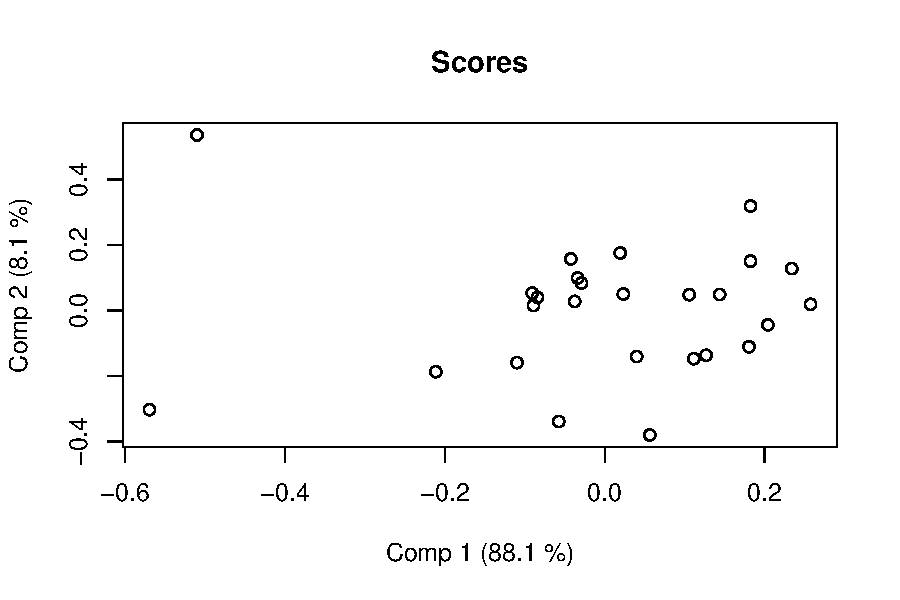
\includegraphics{C:/git/GitHub/multiblock/vignettes/vignette_E_supervised_files/figure-latex/unnamed-chunk-17-1.pdf}

\hypertarget{cvanova}{%
\subsection{CVANOVA}\label{cvanova}}

A CVANOVA model compares absolute or squared cross-validated residuals
from two or more prediction models using ANOVA with \emph{Model} and
\emph{Object} as effects. Tukey's pair-wise testing is automatically
computed.

\begin{Shaded}
\begin{Highlighting}[]
\CommentTok{\# CVANOVA}
\NormalTok{so.pot1 }\OtherTok{\textless{}{-}} \FunctionTok{sopls}\NormalTok{(Sensory[,}\DecValTok{1}\NormalTok{] }\SpecialCharTok{\textasciitilde{}}\NormalTok{ Chemical }\SpecialCharTok{+}\NormalTok{ Compression }\SpecialCharTok{+}\NormalTok{ NIRraw, }\AttributeTok{data=}\NormalTok{potato, }
            \AttributeTok{ncomp=}\FunctionTok{c}\NormalTok{(}\DecValTok{10}\NormalTok{,}\DecValTok{10}\NormalTok{,}\DecValTok{10}\NormalTok{), }\AttributeTok{max\_comps=}\DecValTok{10}\NormalTok{, }\AttributeTok{validation=}\StringTok{"CV"}\NormalTok{, }\AttributeTok{segments=}\DecValTok{10}\NormalTok{)}
\NormalTok{cva }\OtherTok{\textless{}{-}} \FunctionTok{cvanova}\NormalTok{(so.pot1, }\StringTok{"2,1,2"}\NormalTok{)}
\FunctionTok{summary}\NormalTok{(cva)}
\CommentTok{\#\textgreater{} Analysis of Variance Table}
\CommentTok{\#\textgreater{} }
\CommentTok{\#\textgreater{} Response: Residual}
\CommentTok{\#\textgreater{}           Df  Sum Sq Mean Sq F value    Pr(\textgreater{}F)    }
\CommentTok{\#\textgreater{} Model      2  1.0601 0.53007  5.0998  0.009647 ** }
\CommentTok{\#\textgreater{} Object    25 15.1295 0.60518  5.8225 6.511e{-}08 ***}
\CommentTok{\#\textgreater{} Residuals 50  5.1969 0.10394                      }
\CommentTok{\#\textgreater{} {-}{-}{-}}
\CommentTok{\#\textgreater{} Signif. codes:  0 \textquotesingle{}***\textquotesingle{} 0.001 \textquotesingle{}**\textquotesingle{} 0.01 \textquotesingle{}*\textquotesingle{} 0.05 \textquotesingle{}.\textquotesingle{} 0.1 \textquotesingle{} \textquotesingle{} 1}
\CommentTok{\#\textgreater{} Tukey\textquotesingle{}s HSD}
\CommentTok{\#\textgreater{} Alpha: 0.05}
\CommentTok{\#\textgreater{} }
\CommentTok{\#\textgreater{}            Mean G1 G2}
\CommentTok{\#\textgreater{} 2,0,0 0.9696191  A   }
\CommentTok{\#\textgreater{} 2,1,0 0.8208381  A  B}
\CommentTok{\#\textgreater{} 2,1,2 0.6841366     B}
\FunctionTok{plot}\NormalTok{(cva)}
\end{Highlighting}
\end{Shaded}

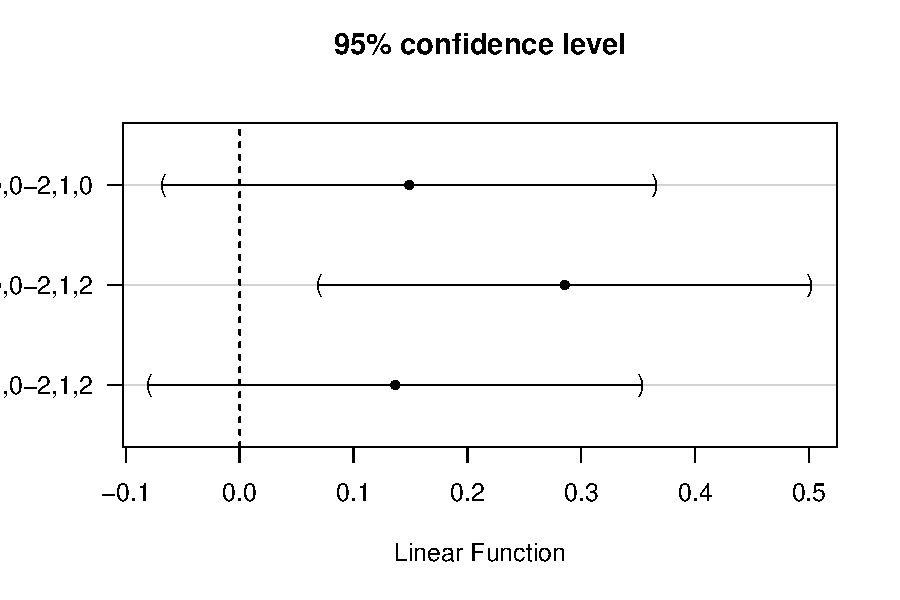
\includegraphics{C:/git/GitHub/multiblock/vignettes/vignette_E_supervised_files/figure-latex/unnamed-chunk-18-1.pdf}

\hypertarget{parallel-and-orthgonalised-partial-least-squares---po-pls}{%
\section{Parallel and Orthgonalised Partial Least Squares -
PO-PLS}\label{parallel-and-orthgonalised-partial-least-squares---po-pls}}

PO-PLS is presented briefly using the \emph{potato} data.

\hypertarget{modelling-3}{%
\subsection{Modelling}\label{modelling-3}}

There are many choices with regard to numbers of components and possible
local and common components. Using automatic selection, the user selects
the highest number of blocks to combine into local/common components,
minimum explained variance and minimum squared correlation to the
response. Manual selection is limited to setting the number of initial
components from the blocks and maximum number of local/common
components.

\begin{Shaded}
\begin{Highlighting}[]
\CommentTok{\# Automatic analysis}
\NormalTok{pot.po.auto }\OtherTok{\textless{}{-}} \FunctionTok{popls}\NormalTok{(potato[}\DecValTok{1}\SpecialCharTok{:}\DecValTok{3}\NormalTok{], potato[[}\StringTok{\textquotesingle{}Sensory\textquotesingle{}}\NormalTok{]][,}\DecValTok{1}\NormalTok{], }\AttributeTok{commons =} \DecValTok{2}\NormalTok{)}

\CommentTok{\# Explained variance}
\NormalTok{pot.po.auto}\SpecialCharTok{$}\NormalTok{explVar}
\CommentTok{\#\textgreater{} $Chemical}
\CommentTok{\#\textgreater{} named numeric(0)}
\CommentTok{\#\textgreater{} }
\CommentTok{\#\textgreater{} $Compression}
\CommentTok{\#\textgreater{} C(1,2), Comp 1 }
\CommentTok{\#\textgreater{}       68.14595 }
\CommentTok{\#\textgreater{} }
\CommentTok{\#\textgreater{} $NIRraw}
\CommentTok{\#\textgreater{} named numeric(0)}
\end{Highlighting}
\end{Shaded}

\begin{Shaded}
\begin{Highlighting}[]
\CommentTok{\# Manual choice of up to 5 components for each block and 1, 0, and 2 blocks,}
\CommentTok{\# respectively from the (1,2), (1,3) and (2,3) combinations of blocks.}
\NormalTok{pot.po.man }\OtherTok{\textless{}{-}} \FunctionTok{popls}\NormalTok{(potato[}\DecValTok{1}\SpecialCharTok{:}\DecValTok{3}\NormalTok{], potato[[}\StringTok{\textquotesingle{}Sensory\textquotesingle{}}\NormalTok{]][,}\DecValTok{1}\NormalTok{], }\AttributeTok{commons =} \DecValTok{2}\NormalTok{,}
                    \AttributeTok{auto=}\ConstantTok{FALSE}\NormalTok{, }\AttributeTok{manual.par =} \FunctionTok{list}\NormalTok{(}\AttributeTok{ncomp=}\FunctionTok{c}\NormalTok{(}\DecValTok{5}\NormalTok{,}\DecValTok{5}\NormalTok{,}\DecValTok{5}\NormalTok{),}
                                                  \AttributeTok{ncommon=}\FunctionTok{c}\NormalTok{(}\DecValTok{1}\NormalTok{,}\DecValTok{0}\NormalTok{,}\DecValTok{2}\NormalTok{)))}
\CommentTok{\# Explained variance}
\NormalTok{pot.po.man}\SpecialCharTok{$}\NormalTok{explVar}
\CommentTok{\#\textgreater{} $Chemical}
\CommentTok{\#\textgreater{} C(1,2), Comp 1   D(1), Comp 1   D(1), Comp 2   D(1), Comp 3 }
\CommentTok{\#\textgreater{}       32.22944   {-}72871.76265   {-}49467.54832        0.00000 }
\CommentTok{\#\textgreater{} }
\CommentTok{\#\textgreater{} $Compression}
\CommentTok{\#\textgreater{} C(1,2), Comp 1 C(2,3), Comp 1 C(2,3), Comp 2 }
\CommentTok{\#\textgreater{}      68.145954       5.504006       7.214911 }
\CommentTok{\#\textgreater{} }
\CommentTok{\#\textgreater{} $NIRraw}
\CommentTok{\#\textgreater{} C(2,3), Comp 1 C(2,3), Comp 2   D(3), Comp 1   D(3), Comp 2   D(3), Comp 3 }
\CommentTok{\#\textgreater{}      32.606459       5.475702    {-}552.399938      15.775647       3.303994 }
\CommentTok{\#\textgreater{}   D(3), Comp 4 }
\CommentTok{\#\textgreater{}       0.000000}
\end{Highlighting}
\end{Shaded}

\hypertarget{scores-and-loadings}{%
\subsection{Scores and loadings}\label{scores-and-loadings}}

Scores and loadings are stored per block. Common scores/loadings are
found in each of the blocks' list of components.

\begin{Shaded}
\begin{Highlighting}[]
\CommentTok{\# Score plot for local (2,3) components}
\FunctionTok{scoreplot}\NormalTok{(pot.po.man, }\AttributeTok{block =} \DecValTok{3}\NormalTok{, }\AttributeTok{labels =} \StringTok{"names"}\NormalTok{)}
\end{Highlighting}
\end{Shaded}

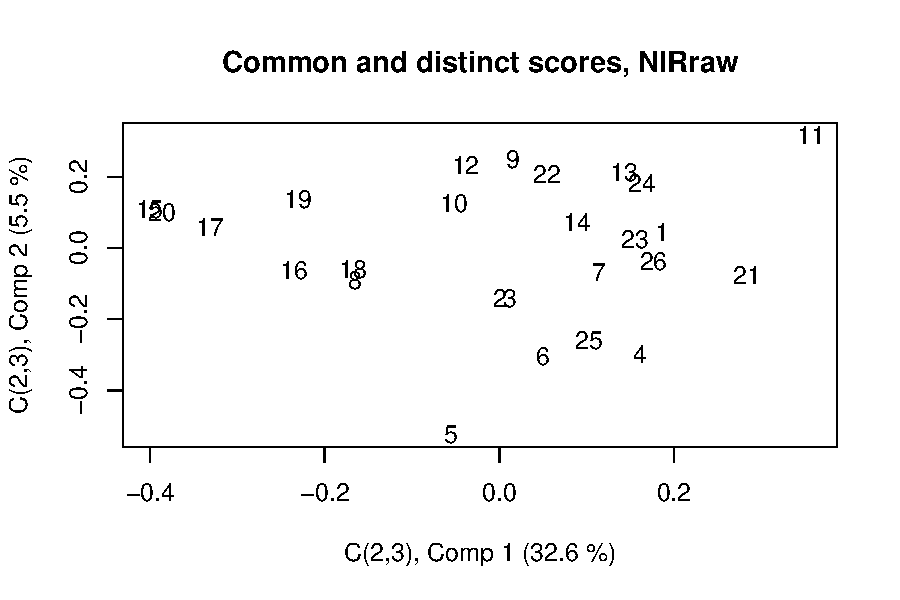
\includegraphics{C:/git/GitHub/multiblock/vignettes/vignette_E_supervised_files/figure-latex/unnamed-chunk-21-1.pdf}

\begin{Shaded}
\begin{Highlighting}[]

\CommentTok{\# Corresponding loadings}
\FunctionTok{loadingplot}\NormalTok{(pot.po.man, }\AttributeTok{block =} \DecValTok{3}\NormalTok{, }\AttributeTok{labels=}\StringTok{"names"}\NormalTok{, }\AttributeTok{scatter =} \ConstantTok{FALSE}\NormalTok{)}
\end{Highlighting}
\end{Shaded}

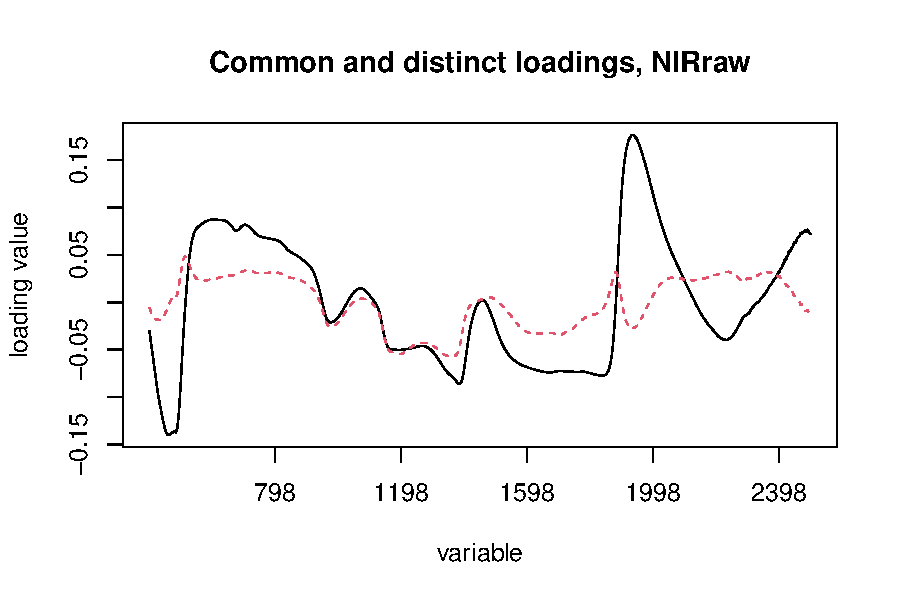
\includegraphics{C:/git/GitHub/multiblock/vignettes/vignette_E_supervised_files/figure-latex/unnamed-chunk-21-2.pdf}

\hypertarget{response-oriented-sequential-alternation---rosa}{%
\section{Response Oriented Sequential Alternation -
ROSA}\label{response-oriented-sequential-alternation---rosa}}

The following example uses the \emph{potato} data to showcase some of
the functions available for ROSA analyses.

\hypertarget{modelling-4}{%
\subsection{Modelling}\label{modelling-4}}

A multi-response two-block ROSA model with up to 10 components in total
is cross-validated with 10 random segments.

\begin{Shaded}
\begin{Highlighting}[]
\CommentTok{\# Model all eight potato blocks with ROSA}
\NormalTok{ros.pot }\OtherTok{\textless{}{-}} \FunctionTok{rosa}\NormalTok{(Sensory }\SpecialCharTok{\textasciitilde{}}\NormalTok{ ., }\AttributeTok{data =}\NormalTok{ potato1, }\AttributeTok{ncomp =} \DecValTok{10}\NormalTok{, }\AttributeTok{validation =} \StringTok{"CV"}\NormalTok{, }\AttributeTok{segments =} \DecValTok{5}\NormalTok{)}
\FunctionTok{print}\NormalTok{(ros.pot)}
\CommentTok{\#\textgreater{} Response Orinented Sequential Alternation , fitted with the CPPLS algorithm.}
\CommentTok{\#\textgreater{} Cross{-}validated using 5 random segments.}
\CommentTok{\#\textgreater{} Call:}
\CommentTok{\#\textgreater{} rosa(formula = Sensory \textasciitilde{} ., ncomp = 10, data = potato1, validation = "CV",     segments = 5)}
\FunctionTok{summary}\NormalTok{(ros.pot)}
\CommentTok{\#\textgreater{} Data:    X dimension: 26 3946 }
\CommentTok{\#\textgreater{}  Y dimension: 26 1}
\CommentTok{\#\textgreater{} Fit method:}
\CommentTok{\#\textgreater{} Number of components considered: 10}
\CommentTok{\#\textgreater{} }
\CommentTok{\#\textgreater{} VALIDATION: RMSEP}
\CommentTok{\#\textgreater{} Cross{-}validated using 5 random segments.}
\CommentTok{\#\textgreater{}        (Intercept)  1 comps  2 comps  3 comps  4 comps  5 comps  6 comps}
\CommentTok{\#\textgreater{} CV           1.778   0.9819   0.8812   0.8756   0.7744   0.9047   1.0309}
\CommentTok{\#\textgreater{} adjCV        1.778   0.9447   0.8468   0.8410   0.7515   0.8734   0.9897}
\CommentTok{\#\textgreater{}        7 comps  8 comps  9 comps  10 comps}
\CommentTok{\#\textgreater{} CV       1.085    1.135    1.135     1.218}
\CommentTok{\#\textgreater{} adjCV    1.051    1.101    1.104     1.184}
\CommentTok{\#\textgreater{} }
\CommentTok{\#\textgreater{} TRAINING: \% variance explained}
\CommentTok{\#\textgreater{}          1 comps  2 comps  3 comps  4 comps  5 comps  6 comps  7 comps  8 comps}
\CommentTok{\#\textgreater{} X          27.82    72.05    82.50    83.10    84.88    87.09    87.24    88.46}
\CommentTok{\#\textgreater{} Sensory    76.53    83.36    84.21    87.91    88.06    88.18    88.17    88.47}
\CommentTok{\#\textgreater{}          9 comps  10 comps}
\CommentTok{\#\textgreater{} X          91.18     92.81}
\CommentTok{\#\textgreater{} Sensory    88.78     88.78}
\end{Highlighting}
\end{Shaded}

\hypertarget{loadings-1}{%
\subsection{Loadings}\label{loadings-1}}

Extract loadings (not used further) and plot two first vectors of
loadings.

\begin{Shaded}
\begin{Highlighting}[]
\NormalTok{loads }\OtherTok{\textless{}{-}} \FunctionTok{loadings}\NormalTok{(ros.pot)}
\FunctionTok{loadingplot}\NormalTok{(ros.pot, }\AttributeTok{comps =} \DecValTok{1}\SpecialCharTok{:}\DecValTok{2}\NormalTok{, }\AttributeTok{scatter =} \ConstantTok{FALSE}\NormalTok{)}
\end{Highlighting}
\end{Shaded}

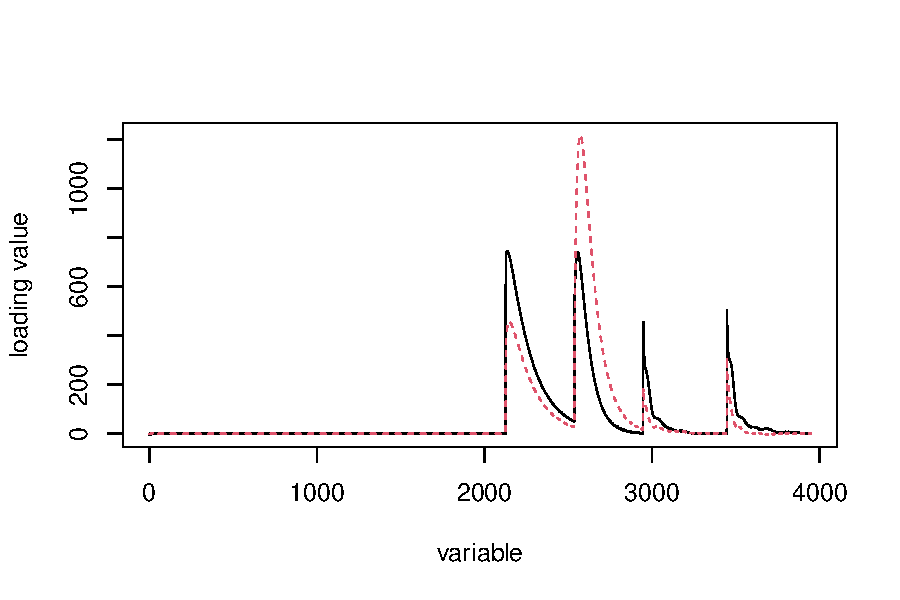
\includegraphics{C:/git/GitHub/multiblock/vignettes/vignette_E_supervised_files/figure-latex/unnamed-chunk-23-1.pdf}

\hypertarget{scores-1}{%
\subsection{Scores}\label{scores-1}}

Extract scores (not used further) and plot two first vectors of scores.

\begin{Shaded}
\begin{Highlighting}[]
\NormalTok{sco }\OtherTok{\textless{}{-}} \FunctionTok{scores}\NormalTok{(ros.pot)}
\FunctionTok{scoreplot}\NormalTok{(ros.pot, }\AttributeTok{comps =} \DecValTok{1}\SpecialCharTok{:}\DecValTok{2}\NormalTok{, }\AttributeTok{labels =} \StringTok{"names"}\NormalTok{)}
\end{Highlighting}
\end{Shaded}

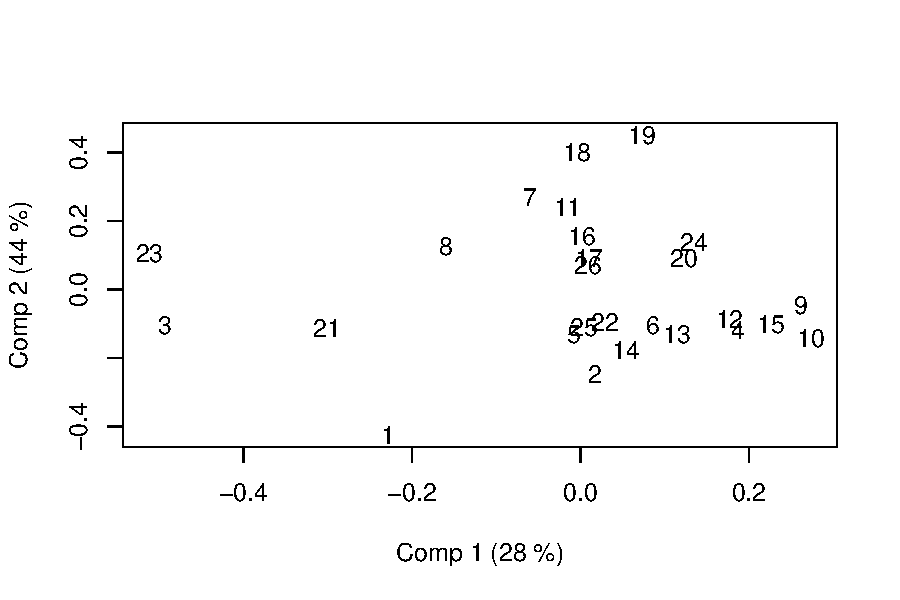
\includegraphics{C:/git/GitHub/multiblock/vignettes/vignette_E_supervised_files/figure-latex/unnamed-chunk-24-1.pdf}

\hypertarget{prediction-1}{%
\subsection{Prediction}\label{prediction-1}}

A three block model is fitted using a single response, 5 components and
a subset of the data. The remaining data are used as test set for
prediction.

\begin{Shaded}
\begin{Highlighting}[]
\CommentTok{\# Model 20 first objects of three potato blocks}
\NormalTok{rosT }\OtherTok{\textless{}{-}} \FunctionTok{rosa}\NormalTok{(Sensory }\SpecialCharTok{\textasciitilde{}}\NormalTok{ ., }\AttributeTok{data =}\NormalTok{ potato1[}\FunctionTok{c}\NormalTok{(}\DecValTok{1}\SpecialCharTok{:}\DecValTok{3}\NormalTok{,}\DecValTok{9}\NormalTok{)], }\AttributeTok{ncomp =} \DecValTok{5}\NormalTok{, }\AttributeTok{subset =} \DecValTok{1}\SpecialCharTok{:}\DecValTok{20}\NormalTok{)}
\NormalTok{testset }\OtherTok{\textless{}{-}}\NormalTok{ potato1[}\SpecialCharTok{{-}}\NormalTok{(}\DecValTok{1}\SpecialCharTok{:}\DecValTok{20}\NormalTok{),]; }\CommentTok{\# testset$Sensory \textless{}{-} NULL}
\FunctionTok{predict}\NormalTok{(rosT, testset, }\AttributeTok{comps=}\DecValTok{2}\NormalTok{)}
\CommentTok{\#\textgreater{}      Sensory}
\CommentTok{\#\textgreater{} 21 2.2151098}
\CommentTok{\#\textgreater{} 22 1.5123048}
\CommentTok{\#\textgreater{} 23 2.3008727}
\CommentTok{\#\textgreater{} 24 1.2001610}
\CommentTok{\#\textgreater{} 25 0.8899352}
\CommentTok{\#\textgreater{} 26 1.2181709}
\end{Highlighting}
\end{Shaded}

\hypertarget{validation-1}{%
\subsection{Validation}\label{validation-1}}

Compute validation statistics; explained variance - R\(^2\) and Root
Mean Squared Error - RMSE(P/CV).

\begin{Shaded}
\begin{Highlighting}[]
\CommentTok{\# Cross{-}validation}
\FunctionTok{R2}\NormalTok{(ros.pot)}
\CommentTok{\#\textgreater{} (Intercept)      1 comps      2 comps      3 comps      4 comps      5 comps  }
\CommentTok{\#\textgreater{}     {-}0.0816       0.6700       0.7342       0.7376       0.7948       0.7199  }
\CommentTok{\#\textgreater{}     6 comps      7 comps      8 comps      9 comps     10 comps  }
\CommentTok{\#\textgreater{}      0.6362       0.5967       0.5594       0.5589       0.4919}
\CommentTok{\# Training}
\FunctionTok{R2}\NormalTok{(ros.pot, }\StringTok{\textquotesingle{}train\textquotesingle{}}\NormalTok{)}
\CommentTok{\#\textgreater{} (Intercept)      1 comps      2 comps      3 comps      4 comps      5 comps  }
\CommentTok{\#\textgreater{}      0.0000       0.7653       0.8336       0.8421       0.8791       0.8806  }
\CommentTok{\#\textgreater{}     6 comps      7 comps      8 comps      9 comps     10 comps  }
\CommentTok{\#\textgreater{}      0.8818       0.8817       0.8847       0.8878       0.8878}

\CommentTok{\# Test data}
\FunctionTok{R2}\NormalTok{(rosT, }\StringTok{\textquotesingle{}test\textquotesingle{}}\NormalTok{, }\AttributeTok{newdata =}\NormalTok{ testset)}
\CommentTok{\#\textgreater{} (Intercept)      1 comps      2 comps      3 comps      4 comps      5 comps  }
\CommentTok{\#\textgreater{}     {-}0.1609       0.3158       0.3289       0.4673       0.4634       0.4574}
\end{Highlighting}
\end{Shaded}

\begin{Shaded}
\begin{Highlighting}[]
\CommentTok{\# Cross{-}validation}
\FunctionTok{RMSEP}\NormalTok{(ros.pot)}
\CommentTok{\#\textgreater{}        (Intercept)  1 comps  2 comps  3 comps  4 comps  5 comps  6 comps}
\CommentTok{\#\textgreater{} CV           1.778   0.9819   0.8812   0.8756   0.7744   0.9047   1.0309}
\CommentTok{\#\textgreater{} adjCV        1.778   0.9447   0.8468   0.8410   0.7515   0.8734   0.9897}
\CommentTok{\#\textgreater{}        7 comps  8 comps  9 comps  10 comps}
\CommentTok{\#\textgreater{} CV       1.085    1.135    1.135     1.218}
\CommentTok{\#\textgreater{} adjCV    1.051    1.101    1.104     1.184}
\CommentTok{\# Training}
\FunctionTok{RMSEP}\NormalTok{(ros.pot, }\StringTok{\textquotesingle{}train\textquotesingle{}}\NormalTok{)}
\CommentTok{\#\textgreater{} (Intercept)      1 comps      2 comps      3 comps      4 comps      5 comps  }
\CommentTok{\#\textgreater{}      1.7093       0.8280       0.6972       0.6792       0.5944       0.5906  }
\CommentTok{\#\textgreater{}     6 comps      7 comps      8 comps      9 comps     10 comps  }
\CommentTok{\#\textgreater{}      0.5877       0.5879       0.5805       0.5726       0.5726}

\CommentTok{\# Test data}
\FunctionTok{RMSEP}\NormalTok{(rosT, }\AttributeTok{newdata =}\NormalTok{ testset)}
\CommentTok{\#\textgreater{} (Intercept)      1 comps      2 comps      3 comps      4 comps      5 comps  }
\CommentTok{\#\textgreater{}       2.435        1.869        1.851        1.649        1.655        1.664}
\end{Highlighting}
\end{Shaded}

\hypertarget{image-plots}{%
\subsection{Image plots}\label{image-plots}}

These are plots for evaluation of the block selection process in ROSA.
Correlation plots show how the different candidate scores (one candidate
for each block for each component) correlate to the winning block's
scores. Residual response plots show how different choices of candidate
scores would affect the RMSE of the residual response. One can for
instance use these plots decide on a different block selection order
than the one proposed automatically by ROSA.

\begin{Shaded}
\begin{Highlighting}[]
\CommentTok{\# Correlation to winning scores}
\FunctionTok{image}\NormalTok{(ros.pot)}
\end{Highlighting}
\end{Shaded}

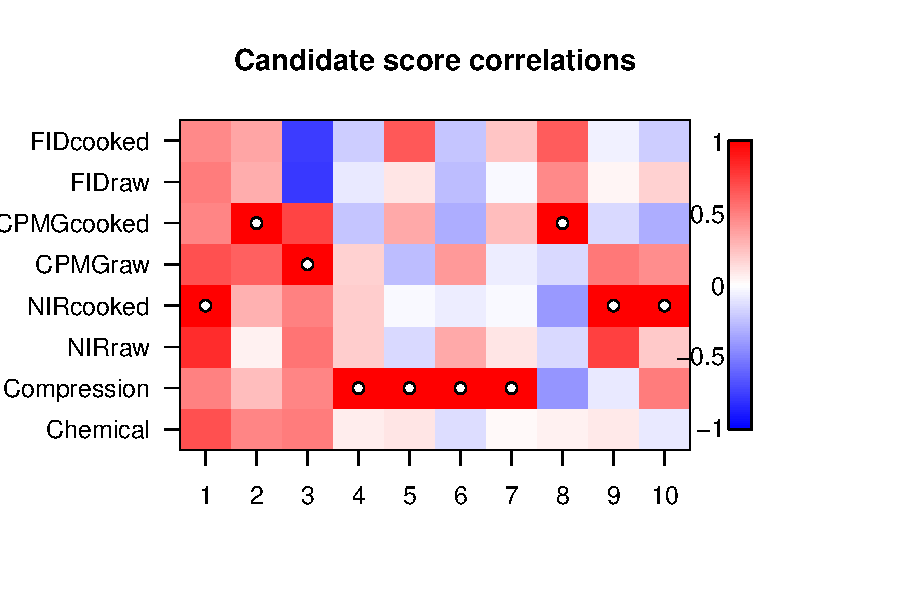
\includegraphics{C:/git/GitHub/multiblock/vignettes/vignette_E_supervised_files/figure-latex/unnamed-chunk-28-1.pdf}

\begin{Shaded}
\begin{Highlighting}[]
\CommentTok{\# Residual response given candidate scores}
\FunctionTok{image}\NormalTok{(ros.pot, }\StringTok{"residual"}\NormalTok{)}
\end{Highlighting}
\end{Shaded}

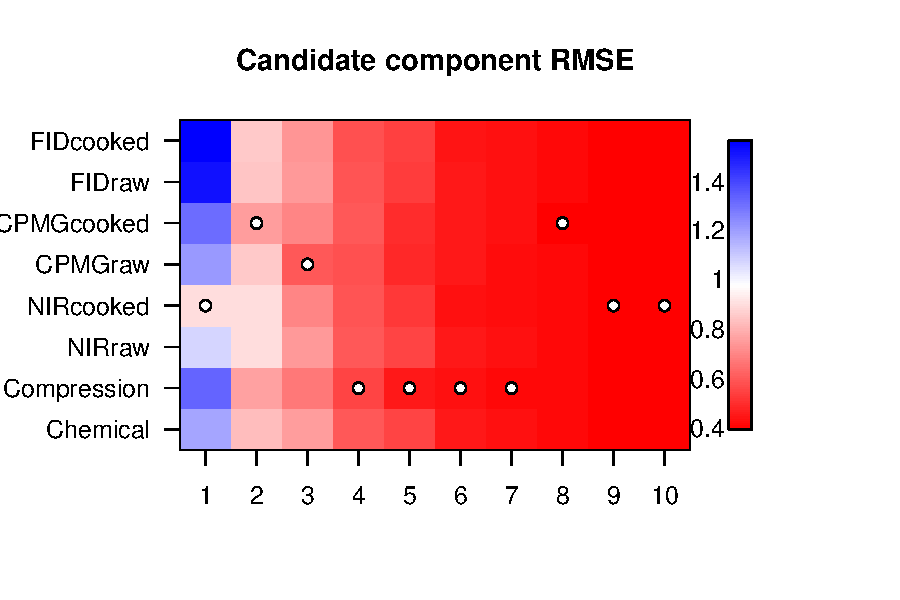
\includegraphics{C:/git/GitHub/multiblock/vignettes/vignette_E_supervised_files/figure-latex/unnamed-chunk-28-2.pdf}

\hypertarget{multiblock-redundancy-analysis---mbrda}{%
\section{Multiblock Redundancy Analysis -
mbRDA}\label{multiblock-redundancy-analysis---mbrda}}

The following example uses the \emph{potato} data to showcase some of
the functions available for mbRDA analyses.

\hypertarget{modelling-5}{%
\subsection{Modelling}\label{modelling-5}}

This implementation uses a wrapper for the \emph{mbpcaiv} function in
the \emph{ade4} package to perform mbRDA. A multi-response 5 component
model is fitted.

\begin{Shaded}
\begin{Highlighting}[]
\CommentTok{\# Convert data.frame with AsIs objects to list of matrices}
\NormalTok{potatoList }\OtherTok{\textless{}{-}} \FunctionTok{lapply}\NormalTok{(potato, unclass)}

\CommentTok{\# Perform mbRDA with two blocks explaining sensory attributes}
\NormalTok{mbr }\OtherTok{\textless{}{-}} \FunctionTok{mbrda}\NormalTok{(potatoList[}\FunctionTok{c}\NormalTok{(}\StringTok{\textquotesingle{}Chemical\textquotesingle{}}\NormalTok{,}\StringTok{\textquotesingle{}Compression\textquotesingle{}}\NormalTok{)], potatoList[[}\StringTok{\textquotesingle{}Sensory\textquotesingle{}}\NormalTok{]], }\AttributeTok{ncomp =} \DecValTok{5}\NormalTok{)}
\FunctionTok{print}\NormalTok{(mbr)}
\CommentTok{\#\textgreater{} Multiblock RDA }
\CommentTok{\#\textgreater{} }
\CommentTok{\#\textgreater{} Call:}
\CommentTok{\#\textgreater{} mbrda(X = potatoList[c("Chemical", "Compression")], Y = potatoList[["Sensory"]],     ncomp = 5)}
\end{Highlighting}
\end{Shaded}

\hypertarget{loadings-and-scores}{%
\subsection{Loadings and scores}\label{loadings-and-scores}}

The \emph{mbpcaiv} wrapper extracts key elements for inspection using
the same format as the rest of this package. The full fitted
\emph{mbpcaiv} object is also available, e.g.~through
\emph{mbr\$mbpcaivObject}.

\begin{Shaded}
\begin{Highlighting}[]
\CommentTok{\# Extract and view loadings}
\NormalTok{lo\_mbr }\OtherTok{\textless{}{-}} \FunctionTok{loadings}\NormalTok{(mbr)}
\CommentTok{\#\textgreater{} Warning in loadings.multiblock(mbr): No global/consensus loadings available.}
\CommentTok{\#\textgreater{} Returning block 1 loadings.}
\FunctionTok{print}\NormalTok{(}\FunctionTok{head}\NormalTok{(lo\_mbr))}
\CommentTok{\#\textgreater{}           Comp 1      Comp 2     Comp 3     Comp 4     Comp 5}
\CommentTok{\#\textgreater{} PEU  {-}0.11801083  0.45883565 {-}1.7606202 {-}0.1936109 {-}2.3704052}
\CommentTok{\#\textgreater{} Sta.  1.02113965 {-}2.99539512  1.4968283  4.6426038 {-}7.6478047}
\CommentTok{\#\textgreater{} TotN  0.50084474 {-}1.40837541  1.0571404  1.8302797 {-}1.7127587}
\CommentTok{\#\textgreater{} Phy.  0.24298763  0.27655908  0.3695837  0.4462580 {-}0.7461178}
\CommentTok{\#\textgreater{} Ca    0.02050271 {-}0.04647818  0.1311656  0.6243666 {-}0.9713523}
\CommentTok{\#\textgreater{} Mg   {-}0.21159305  1.41437345 {-}0.6562877 {-}1.4166021  2.0111970}
\CommentTok{\# Plot scores}
\FunctionTok{scoreplot}\NormalTok{(mbr, }\AttributeTok{labels =} \StringTok{"names"}\NormalTok{)}
\end{Highlighting}
\end{Shaded}

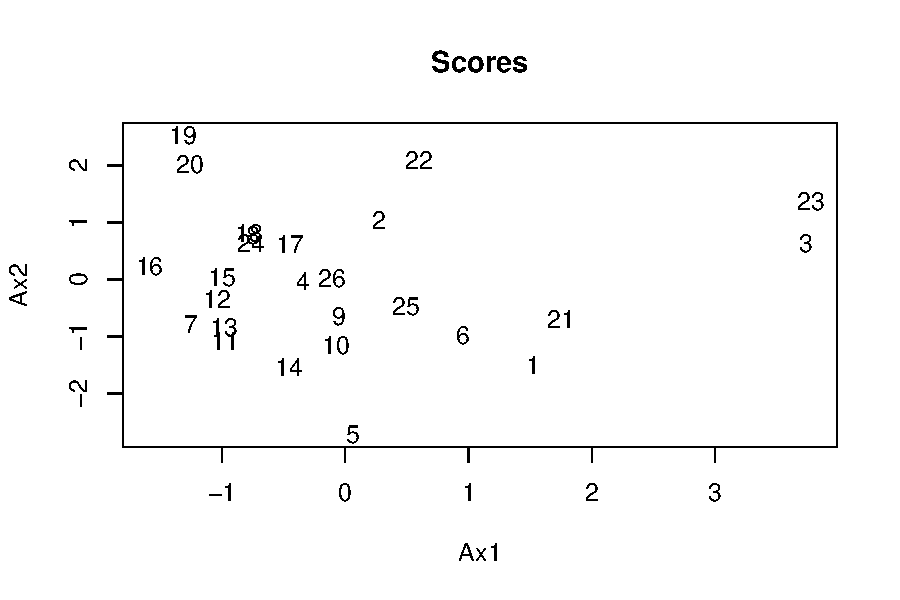
\includegraphics{C:/git/GitHub/multiblock/vignettes/vignette_E_supervised_files/figure-latex/unnamed-chunk-30-1.pdf}

\end{document}
